\documentclass[twoside,12pt,parskip=half-]{scrartcl}
\raggedbottom

% Für TODO nach %XXX suchen.
% Regeln: du statt euch in sätzen verwenden um Leser direkt anzusprechen
% Darauf achten, dass Seitenzahl durch 4 teilbar ist damit es am ende keine leeren seiten gibt 
% fs.lmu.de/gaf/impurity :) 
% Schreibweisen: E-Books, E-Mail, Webseite, Campuskennung, VPN-Client, BAföG, WLAN, UniWorX

%\usepackage[paperwidth=152mm, paperheight = 214mm,twoside, left=17mm, right=17mm, top=22mm, bottom=27mm, bindingoffset=5mm]{geometry}
\usepackage[a4paper,left=17mm, right=17mm, top=22mm, bottom=27mm, bindingoffset=5mm,twoside]{geometry}
\usepackage[ngerman]{babel}

\usepackage{xcolor}
\usepackage{dtklogos}
\usepackage{setspace}
\usepackage{multicol}
\usepackage{tocloft}
\usepackage{eurosym}
% implied by XeLaTeX
%\usepackage[utf8]{inputenc}
\usepackage{wrapfig}
\usepackage{microtype}
\usepackage{graphicx}
\usepackage{multirow}
\usepackage{tikz}
\usetikzlibrary{positioning}
\usetikzlibrary{shapes}
\graphicspath{{img//}}
\usepackage[hidelinks]{hyperref}
\usepackage[absolute]{textpos}

% redefine header/footer
\usepackage{scrpage2}
\ihead{}
\ohead{\rightmark}
\chead{}
\ifoot{}
\ofoot{\thepage}
\cfoot{Ersti-Einstein WS 2012/13}
\pagestyle{scrheadings}
\automark[section]{section}

% no section numbers in heads
\renewcommand\sectionmark[1]{\markright{#1}}
\newcommand{\emd}{\textendash}

% compact toc
\setlength{\cftbeforesecskip}{0pt}
\setcounter{tocdepth}{2}

% lmu fonts
\usepackage[T1]{fontenc}
%\usepackage[defaultsans]{droidsans}
%\renewcommand*\familydefault{\sfdefault}
\usepackage{fontspec}
\linespread{1.05}
\usepackage{microtype}
\setmainfont[Ligatures=TeX,SmallCapsFont={* SC}]{LMU CompatilText}

\usepackage[babel=once]{csquotes}
\defineshorthand{"`}{\openautoquote}
\defineshorthand{"'}{\closeautoquote}
\DeclareQuoteStyle[quotes]{german}{„}{“}{‚}{‘}

\newcommand{\skiptobottom}{\vspace*{0pt plus 1filll}}

\usepackage{endnotes} %Für alle URLs am Ende des Einsteins
\def\enotesize{\fontsize{9}{12}}
\def\notesname{URLs}
\usepackage{tabularx}
\newcolumntype{L}{>{\raggedright\arraybackslash}p{0.3\textwidth}} % linksbündig mit Breitenangabe

%\usepackage[hyphens]{url}
\usepackage{url}
\urlstyle{same}

%\hypersetup{colorlinks=false,urlbordercolor=black,pdfborderstyle={/S/U/W 0.5}}



\mathchardef\UrlBreakPenalty=100
\mathchardef\UrlBigBreakPenalty=100


%\setlength{\parindent}{0cm}
%\setlength{\parskip}{-1pt plus 0.0pt minus 0.0pt}
%\setlength{\parsep}{0pt plus 0.0pt minus 0.0pt}




\begin{document}
% ---- begin formats




\renewenvironment{itemize}
{
    \begin{list}{$\circ$ \ }{}
        \setlength{\topsep}{0pt}
        \setlength{\parskip}{0pt}
        \setlength{\partopsep}{0pt}
        \setlength{\parsep}{0pt}         
        \setlength{\itemsep}{1pt} 
}
{
    \end{list} 
}




\hyphenation{Im-ma-tri-ku-la-tions-be-schei-ni-gung}

% ---- end formats

%\frontmatter

\begin{titlepage}
\thispagestyle{empty}
\begin{textblock*}{\paperwidth}(0mm,0mm)
   \noindent
\includegraphics[width=\paperwidth,height=\paperheight]{titel}
\end{textblock*}
\mbox{}
\end{titlepage}



\newpage

\thispagestyle{empty}
\skiptobottom
\section*{Impressum}

\begin{tabular}{ l l l l }
  Redaktion &Andreas Fichtner& Satz & Julia, Chris\\
  &Max Klinger& & \\
  &Tobias Munzert & Toolchain & Google Docs, Emacs,\\
  &Julia Ringler && \XeLaTeX\\
 "`Lektorat"' & Christian Neukirchen & Druck & Copy World München\\
  & Lukas Milles && Theresienstr. 46 \\
  & &&80333 München \\
  Stand & \today & Auflage&1000\\
  \\
  V.i.S.d.P. & Max Klinger\\ 
  \\
  Adresse &\multicolumn{2}{l}{Gruppe Aktiver Fachschaftika}\\
  & Redaktion Einstein\\
&\multicolumn{3}{l}{Theresienstr. 39, B037}\\
&80333 München\\
  \\
Telefon&089 / 2180\emd{}4382 & &
\hfill\multirow{5}{*}{
\includegraphics[width=1in]{gaf.png}} \\
Telefax&089 / 2180\emd{}4391\\
&\\
& \url{gaf@fs.lmu.de}\\
&\url{einstein@fs.lmu.de}\\
&\url{gumbel@fs.lmu.de}\\
&\\
&\url{gaf.fs.lmu.de}\\
& \url{facebook.com/gaflmu}\\
&		\\
IRC & \url{#gaf} auf freenode & 	&	$\quad$ Link: gaf.fs.lmu.de\\
&\\
Einstein online	&	\url{gaf.fs.lmu.de/erstiinfos/ersti-einstein}
\end{tabular}

\clearpage


\setcounter{page}{1}

\vspace*{0.02cm}
%\footnotesize
\tableofcontents
%\normalsize
\clearpage

\def\mail#1{\url{#1}}

\section{Über \ldots}

\subsection{\ldots{} dieses Heft}

Bei der ganzen Informationsflut, die in der ersten Unizeit auf dich
einstürzt, hoffen wir dir mit unserem \emph{Ersti-Einstein} einen
kleinen Ratgeber an die Hand zu geben.  Der Ersti-Einstein bündelt
Wichtiges, erklärt dir Nichtoffensichtliches, und versucht bei vielen
Problemen zumindest erste Lösungsansätze zu bieten.

Da wir nicht mehr alle Probleme, die ein Ersti hat, nachvollziehen
können, und jedes Jahr neue Probleme gefunden werden, würden wir uns
freuen, wenn du uns fehlende Informationen unter
\mail{einstein@fs.lmu.de} mitteilst.


\subsection{\ldots{} uns}

Wir sind die GAF -- Gruppe Aktiver Fachschaftika -- ein
Zusammenschluss der Fachschaften der Fachbereiche
Mathematik,
Physik
und Informatik (also auch Wirtschaftsmathe, Medieninfo und
Meteorologie), sowie den dazugehörigen Lehramtsstudiengängen.

\paragraph{Was ist eine Fachschaft?}

Eine Fachschaft sind alle Studenten in einem Studiengang, das heißt die Fachschaft Physik besteht zum Beispiel aus \emph{allen} Studenten (ob ihr wollt oder nicht), die in Physik eingeschrieben sind.

Wenn man von \emph{der Fachschaft} spricht, meint man normalerweise die Aktiven,
zum Beispiel die Organisatoren der O-Phase.

\paragraph{Was macht die Fachschaft?}
\begin{itemize}
\item Repräsentation studentischer Interessen auf allen Ebenen, d.h. in Universitätsgremien z.B. dem Fakultätsrat, der Studiengebührenkommission oder Berufungskommissionen für neue Professoren \ldots
\item Verwaltung alter Klausuren, Prüfungsprotokolle und allem Anderen, was beim Studium hilft.
\item Information (O-Phase) und Beratung. Wenn du Fragen hast und nicht mal weißt, wen du fragen sollst, frag' uns.
\item Bespaßung: Wir organisieren Partys und andere Aktionen (Casinoabend, Jazzabend, Fakultätsfest, \ldots), damit auch der soziale Aspekt an der Uni nicht zu kurz kommt.
\item Anlaufstelle für Fragen aller Art; Sammeln von Meinungen für die Fakultät und Informationen aus der Fakultät, die wir an dich weiter leiten.
\end{itemize}

\paragraph{Wie machen die das?}
Die Fachschaft an sich bekommt Geld, das aber nur zum Nutzen der
Studenten eingesetzt werden darf, d.h. diejenigen, die in der
Fachschaft aktiv sind, tun dies ehrenamtlich und unentgeltlich.

\clearpage

\paragraph{Ich will mitmachen! Wie?}\label{mitmachen}\hfill\\

Komm einfach vorbei:
\begin{itemize}
	\item ins Fachschaftszimmer (Theresienstr., B037)
	\item zur Fachschaftssitzung (Termine unter \url{gaf.fs.lmu.de/wir/fachschaftssitzung})
\end{itemize}
oder sprich uns bei der O-Phase an.


\paragraph{Wie kann ich euch erreichen?}\label{gafKontakt}\hfill\\[1em]

\begin{tabular}{ l l l l }
Telefon&089 / 2180\emd{}4382\\
Telefax&089 / 2180\emd{}4391\\
&\\
&\mail{gaf@fs.lmu.de}\\
&\mail{einstein@fs.lmu.de}\\
&\mail{gumbel@fs.lmu.de}\\
&\\
&\url{gaf.fs.lmu.de}\\
&\url{facebook.com/gaflmu}\\
&\\
IRC & \url{#gaf} auf freenode
\end{tabular}

\paragraph{Andere Fachschaften}
\begin{itemize}
	\item \textbf{Medieninformatik:} \url{mi.fs.lmu.de} und \url{facebook.com/FS.Medieninformatik.LMU}
	\item \textbf{Bioinformatik:} \url{www.bioinformatik-muenchen.com/bioinfocom/fachschaft/}
	\item \textbf{Meteorologie:} \url{www.meteo.physik.lmu.de/~studmet}
\end{itemize}

\skiptobottom
\centerline{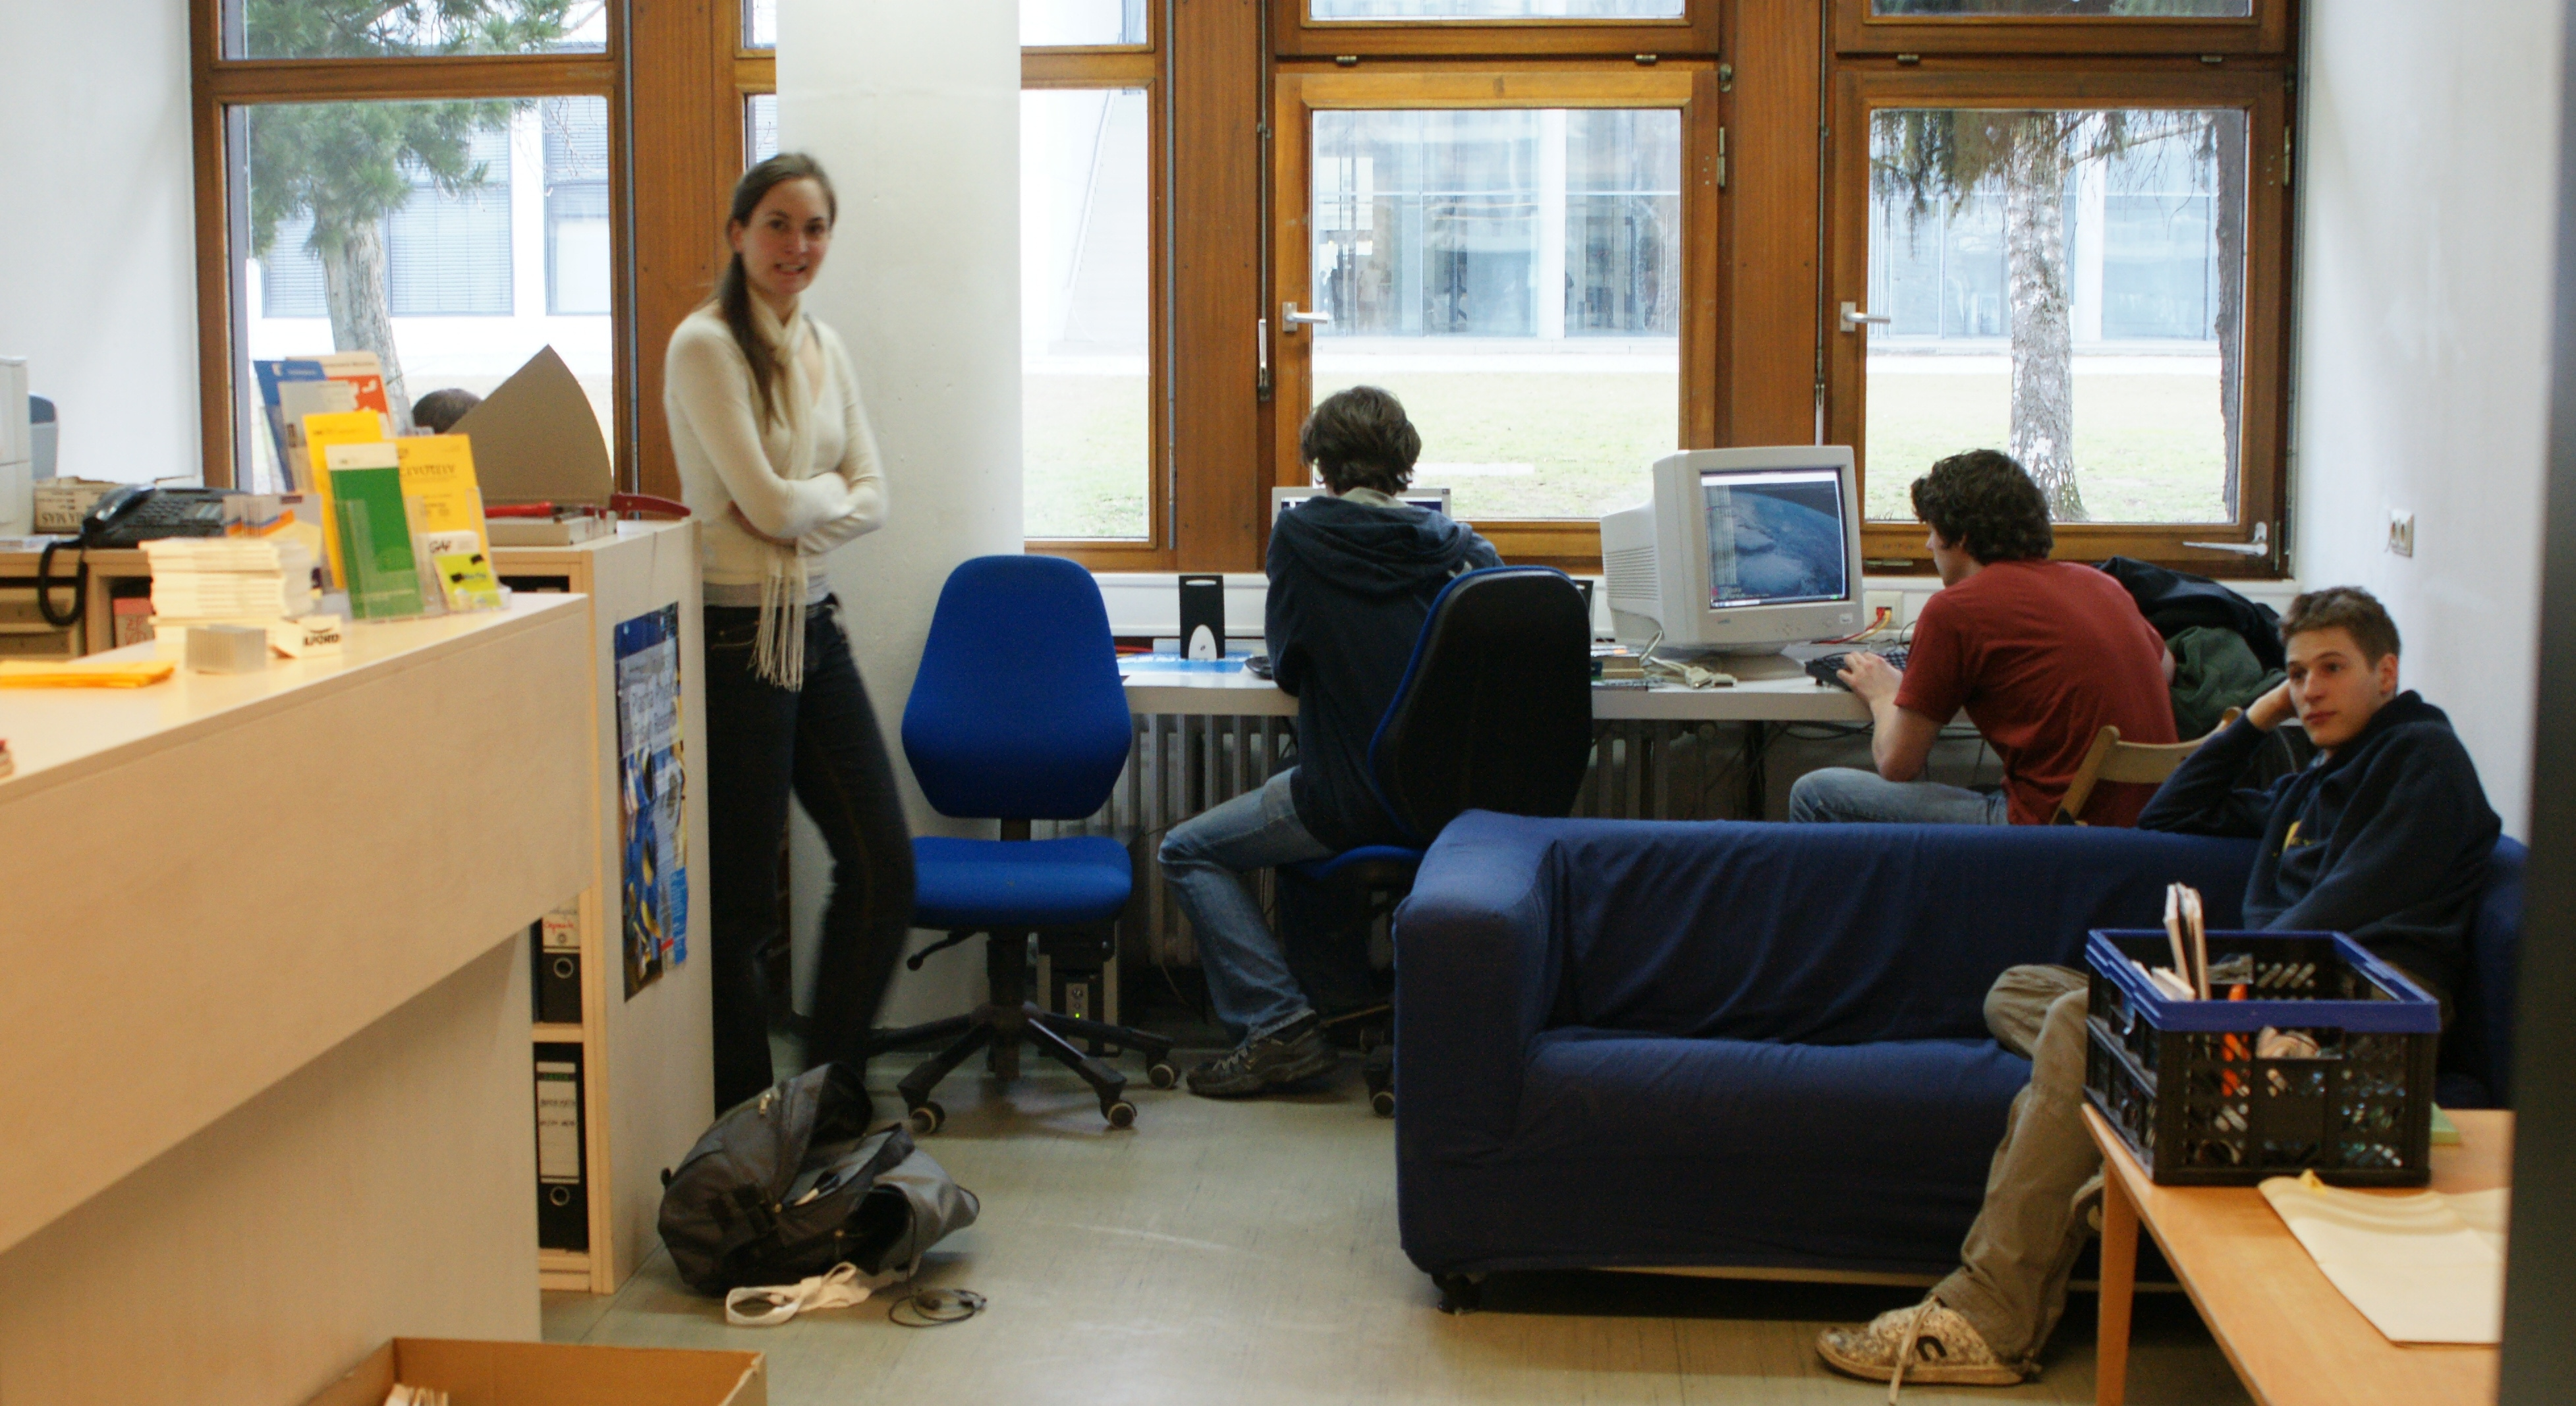
\includegraphics[width=0.8\textwidth]{aktive-fachschaft_print}}

\clearpage

\section{Computer und Internet}

\subsection{Online-Dienste der LMU}

\paragraph{Online-Selbstbedienungsfunktionen}\hfill\\
\url{www.lmu.de/studium/studium_aktuell/neuigkeiten/studkanz/system.html}
\begin{itemize}
	\item Bescheinigungen: Immatrikulation, Studienverlauf, gezahlte Beiträge
	\item Adress-/ Telefonnummernänderung
	\item Formular zur Prüfungsanmeldung
\end{itemize}

\paragraph{CAMPUS LMU}\hfill\\
\url{campus.lmu.de} oder \url{www.portal.lmu.de}
\begin{itemize}
	\item Aktivierung der Campuskennung
	\item Zugang zum E-Mailaccount und Benutzerkonto (An-/Abmeldung von Newslettern der LMU)
	\item Zugang zum LSF (Vorlesungsverzeichnis)
	\item Personalisierbare Startseite mit Feldern wie Veranstaltungen, Mensa, Quicklinks etc.
\end{itemize}

\paragraph{Vorlesungsverzeichnis}\hfill\\
\url{www.lsf.lmu.de}
\begin{itemize}
	\item Übersicht über alle Veranstaltungen der LMU
	\item Stundenplan-Tool (etwas merkwürdig zu bedienen)
	\item Anmeldung zu Kursen und Klausuren (BWL, VWL)
        \item Notenauszug, nicht immer aktuell (Physik)
\end{itemize}

\paragraph{UniWorX (Informatik, Medieninformatik)}\hfill\\
\url{uniworx.ifi.lmu.de}
\begin{itemize}
	\item Anmeldung zu Kursen und Klausuren im Bereich Informatik
	\item Abgabe von Übungsblättern
\end{itemize}

\paragraph{Prüfungsverwaltungs- und Informationssystem (PVI)}\hfill\\
\url{pvineu.ifi.lmu.de}
\begin{itemize}
	\item Notenabfrage für Informatik und Medieninformatik
\end{itemize}

\clearpage

\subsection{E-Mail}
Damit du nicht unterfordert wirst, besitzt du direkt von Anfang an zwei verschiedene E-Mailadressen. Bei beiden E-Mailadressen ist es möglich eine Weiterleitung einzurichten.\\

Die erste Adresse besitzt jeder Student der LMU, während die Zweite für alle Nutzer der CIP-Pools ist.

\paragraph{Für alle LMU-Studierende}
\begin{itemize}
	\item <vorname.nachname>@campus.lmu.de (bzw. was ihr angegeben habt)
	\item Webmail unter: \url{mailbox.portal.uni-muenchen.de}
\end{itemize}

\paragraph{Informatik und MedienInformatik}\hfill\\
Sollte unbedingt weitergeleitet oder abgerufen werden, da hierüber der Großteil des Informatik-Mailverkehrs abläuft. Insbesondere das Abgabesystem Uniworx schickt euch Informationen der Dozenten und Korrekturergebnisse an diese Adresse.
\begin{itemize}
	\item <accountname>@cip.ifi.lmu.de
	\item Webmail unter: \url{webmail.ifi.lmu.de}
	\item Infos unter: \url{www.rz.ifi.lmu.de/Dienste/Mailsystem.html}
	\item Beantragung der Kennung: \url{www.rz.ifi.lmu.de}
\end{itemize}

\paragraph{Physik und Meteorologie}\hfill\\
An diese Adresse werden Ankündigungen des Prüfungsamtes und
Physik-Newsletter gesendet.

\begin{itemize}
	\item <vorname.nachname>@physik.uni-muenchen.de
	\item Webmail unter \url{webmail.physik.uni-muenchen.de}
	\item Infos unter \url{it.physik.uni-muenchen.de/dienste/kommunikation/e-mail}
        \item Passwort wie bei \url{campus.lmu.de}.
\end{itemize}

\paragraph{Mathematik und Wirtschaftsmathematik}
\begin{itemize}
	\item <seltsameKombination>@math.lmu.de
	\item Infos nur aus dem CIP-Pool abrufbar, Einführung/ Beantragung E-Mailadresse bei Herrn Spann (Anmeldung in der Theresienstr., B124)
	\item Weiterleitung über Shell-Kommando \verb|echo "neue Adresse" >~/.forward|
\end{itemize}

\subsection{CIP-Pools}
Computer, soziale Kontake und Drucken (600 Seiten/Semester kostenlos).\\

\begin{tabular}{l p{10cm}}
\textbf{Mathematik}	&	Theresienstr., BU135 und BU136, \newline Wendeltreppe nach unten\\

\textbf{Physik, Meteorologie}	&	Schellingstr. 4 Erdgeschoss, H037 und H022\\
\textbf{Medieninformatik, Informatik}	&	Oettingenstr. 67, BU102, LU112, LU114 und LU117 (Keller und Barracken)\\
\textbf{Medieninformatik zusätzlich}	&	Amalienstr. 17, EG\\
\textbf{Für alle*}	&	Theresienstr., 1. Stock B115\newline
\footnotesize{$^*$Physik: arbeiten, nicht drucken; \newline Informatik: drucken, nicht arbeiten}

\end{tabular}


\subsection{Internet: WLAN, VPN und Eduroam}

Um mit deinem Laptop in der Uni ins Internet zu gehen, brauchst du
deinen Campus-Account. Damit lassen sich die WLAN-Services des
Leibniz-Rechen\-zentrums (LRZ) nutzen.

\paragraph{Eduroam}
Wir empfehlen dir, das WLAN mit dem Namen (SSID) \emph{eduroam}, auf deinen Geräten einzurichten. Mit diesem einmal eingerichteten Eduroam kannst du weltweit an vielen Universitäten und Forschungsinstituten automatisch das dortige WLAN nutzen. Unter \url{lrz.de/services/netz/mobil/eduroam} findest du ausführliche Anleitungen für die meisten Betriebssysteme und Smartphones.
(Die benötigte LRZ-Kennung findest du in deinem Campus-Account unter 'Benutzerkonto' $\rightarrow$ 'E-Mail-Einstellungen'.)

Die Anleitung \emph{Windows (alt)} bezieht sich übrigens einfach auf
Windowsversionen vor Windows 7.

Falls du nun in der Uni sitzt und dich fragst, wie du ohne Internet
die Anleitung durchlesen oder deine LRZ-Kennung herausfinden sollst:

\paragraph{LRZ}

Außer eduroam gibt es noch die Möglichkeit, das Netz mit der SSID
\emph{lrz} zu verwenden. \emph{lrz} ist zunächst ein unverschlüsseltes
Netzwerk, das nur den Zugriff auf die Website des
Leibnitz-Rechenzentrums gestattet. Von dort kannst du dir dort die
vorkonfigurierte Clientsoftware AnyConnect herunterladen, welche dich
nach Anmelden mit deiner Campuskennung in ein VPN (Virtual Private
Network) des LRZ einbucht. Aus Netzwerksicht verhält sich dein Rechner
dann wie alle anderen Rechner im Münchener Wissenschaftsnetz. So
kannst du nicht nur normal surfen, sondern auch von außen auf das
Münchner Wissenschaftsnetz zugreifen und zum Beispiel bestimmte
Artikel aus der Bibliothek lesen.

Die Clientsoftware ist übrigens außerhalb der Uni praktisch, um deine
HTTP-Verbindungen zu verschlüsseln, etwa wenn du dich in einem
ungeschützen WLAN befindest.

\paragraph{Microsoft DreamSpark}
Studenten der Physik und Informatik (auch im Nebenfach) bekommen über
Microsoft DreamSpark (früher MSDNAA) viele Microsoftproduktlizenzen
gratis, darunter Windows, Visual Studio und viele
Microsoft Office-Komponenten, jedoch \textbf{nicht} Word, Excel und PowerPoint.

\paragraph{Proxyeinrichtung}

Um E-Books, Paper, und wissenschaftliche Journale der Uni-Bib
herunterladen zu können, benötigst du einen Proxyzugang. Dazu musst du
entweder im MWN (Münchner Wissenschaftsnetz, z.B. im CIP) sitzen oder
mittels dem VPN-Client so wirken als ob und dann einen Proxy in deinem
Browser eintragen. Wie man das macht wird hier erklärt:
\url{www.ub.uni-muenchen.de/?id=2402}.

Einfacher gehts seit Neustem mit dem Easyproxy:\\
\url{www.ub.uni-muenchen.de/elektronische-medien/hilfe-anleitungen/easyproxy/}

\clearpage


\section{Vorlesungszeit}

\subsection{Wie bastelt man einen Stundenplan?}

Das Vorlesungsverzeichnis findest du unter: \url{www.lsf.lmu.de}

Auf den Fakultätsseiten gibt es zum Teil noch eine kommentierte
Version. In der Aktualität wechseln sich die beiden Seiten ab, meist
ist die kommentierte Version jedoch vollständiger.

Die Erstellung über das lsf ist sehr kompliziert und weniger
empfehlenswert.  Wichtig ist, dsas du explizit auf ``Plan Speichern''
klickst!  Papier vergisst nichts.

\begin{itemize}
	\item Sortiere nach verbindlichen und empfohlenen Veranstaltungen.
	\item Plane erst obligatorische Veranstaltungen (Studienplan).
	\item Beachte Lehrveranstaltungszyklen (Was baut aufeinander auf?)
	\item Beachte, ob eine Lehrveranstaltung nicht in jedem
          Semester angeboten (z.b. nur jährlich) wird und ob
          Vorlesungen und Seminare oder Übungen im Zusammenhang
          stehen.
	\item Plane Lehrveranstaltungen in einem Umfang von höchstens 20 Semesterwochenstunden, denn Übungen, Tutorien, Selbststudienzeiten sowie Vor- und Nachbereitungen sind in jedem Fall notwendig.
	\item Beachte Wege und Fahrzeiten zwischen den Vorlesungen.
	\item Überprüfe den Stundenplan nach der ersten Vorlesungswoche in Bezug auf Mach- und Brauchbarkeit deines Plans.
	\item Erstelle darüber hinaus einen Semesterplan, in dem alle Termine, Fristen, Aktivitäten vermerkt sind, wie Rückmeldefristen, Klausuren, Referate oder Vorbereitungszeiten für Prüfungen.
	\item Schaue über den Tellerrand hinaus und tief in den Teller hinein. Die LMU bietet eine Vielzahl von Studiengängen an. Suche dir ruhig auch einmal etwas heraus, was dich zwar interessiert, du aber nicht in dein Studium einbringen kannst (von Arabistik bis Zoologie\ldots).
	\item Berücksichtige auch zusätzliche Veranstaltungen, wie beispielsweise Sprachen lernen, Computerkurse, Sport o.ä.
\end{itemize}


\subsection{Zusatz-Angebote}
\begin{itemize}
	\item Fremdsprachen: \url{www.sprachenzentrum.lmu.de}
	\item Ringvorlesung: \url{www.lmu.de/ringvorlesung}
	\item Studium Generale: \newline \url{www.lmu.de/studium/studienangebot/lehrangebote/studium_generale}
	\item LMU PLUS Seminare: \url{www.frauenbeauftragte.lmu.de/plus/plus_veranstaltungen}
	\item Soft Skills, Bewerbungstraining: \url{s-a.uni-muenchen.de} und \url{www.jobline.lmu.de}
	\item Soft Skills an der TUM: \newline \url{www.cvl-a.de/index.php?option=com_content&view=article&id=24}
\end{itemize}


\clearpage


\subsection{Zentraler Hochschulsport (ZHS)}
Für den körperlichen Ausgleich zum Studium kann man in kostspielige Fitnesscenter gehen oder aber eine der vielen interessanten Sportarten, wie z.B. Fechten, Segeln oder Bergsteigen ausprobieren, die vom ZHS zu einem relativ günstigen Preis (ab 7,50~€ pro Semester) angeboten werden. Der Großteil des Angebots findet auf dem Olympiagelände statt und ist -- abgesehen vom Fahrrad -- am besten mit der U3 (Haltestelle Olympiazentrum) und einem kurzen Fußmarsch durchs Olympische Dorf zu erreichen.

Das komplette Sportangebot könnt ihr der Homepage (\url{zhs-muenchen.de}) und dem Hochschulsportheft entnehmen, das zu Semesterbeginn unter anderem im Gumbel ausliegt.

Meistens ist eine Onlineanmeldung verpflichtend, damit du an den
Kursen teilnehmen darfst. Bringe deine Anmeldebestätigung ausgedruckt
mit. Für die Teilnahme brauchst du einen ZHS-Ausweis der
entsprechenden Kategorie mit gültigen Sportmarken, welche online
gebucht werden müssen. Danach musst du dir mit ausgedruckter
Buchungsbestätigung, Studentenausweis, Lichtbildausweis und Passfoto
in der ZHS einen Ausweis erstellen lassen und die entsprechenden
Marken besorgen. In der ersten Woche des Semesters ist das auch in der
Innenstadt (Schellingstr. 3) möglich.



\subsection{Essen}

Die verschiedenen Mensen des Studentenwerks mit Speiseplänen findet ihr unter\\ \url{studentenwerk-muenchen.de/mensa}. Zum Bezahlen braucht man eine Mensakarte, die man dort erwerben und aufladen kann.

In manchen Universitätsgebäuden ist darüber hinaus eine Cafeteria zu finden mit ähnlich preiswerten Essensangebot (Hauptgebäude (HGB) Nordhof, Schellingstr. 1. Stock, Oettingenstr. Keller, Giselastr. Mensagebäude).

Auch wenn du dir selbst ein Bild machen solltest, hier vorab ein Testbericht der Süddeutschen zu den verschiedenen Mensen:
sueddeutsche.de/muenchen/uni-mensen-im-test-\newline voll-auf-die-geschmacksnerven-1.32268

Wenn dir das Essen in den Mensen auf Dauer zu langweilig wird und du trotzdem nicht viel Geld ausgeben willst, hier ein paar Geheimtipps:

\begin{itemize}
	\item \textbf{Finanz- bzw. Landwirtschaftsministerium} (Odeonsplatz 4 bzw. Ludwigstr. 2): Ausschließlich für Mitarbeitern und Studenten. Darum musst du auch einen gültigen (Münchener) Studentenausweis und manchmal zusätzlich deinen Personalausweis vorzeigen. Es gibt täglich wechselnde Gerichte zu Preisen von 3,90~€ bis 6,00~€, jeden Mittwoch ist der allseits beliebte “Schnitzeltag” (4,10~€ mit Salat und Beilage).

	\item \textbf{HFF-Mensa (Hochschule für Film und Fernsehen)}
          (Bernd-Eichinger-Platz 1, gegenüber der TUM-Mensa): Etwas
          teurer als unsere Mensa, dafür aber besser.
\end{itemize}


\clearpage

\section{Vorlesungsfreie Zeit}

Heißt deshalb nicht Ferien sondern vorlesungsfreie Zeit, weil man hier endlich die Zeit hat Klausuren zu schreiben, zu lernen und Blockseminare sowie Praktika zu besuchen. Die Uni kalkuliert dies so, dass man am Ende wieder 6 Wochen Ferien, wie normale Arbeitnehmer auch, hat.

\subsection{Klausuren, Protokolle und Skripte}
Wir von der GAF sammeln Altklausuren, Skripte und mündliche Prüfungsprotokolle. Die meisten Prüfungsprotokolle findest du online: \url{gaf.fs.lmu.de/klausuren}. Benutzernamen und Passwort könnt ihr bei uns in der GAF erfragen.

Damit auch künftige Generationen davon profitieren schickt bitte alles
was ihr in die Hände bekommt (sofern noch nicht vorhanden) an uns.
Wenn du in einer Klausur sitzt, in der die Offiziellen euch Strafen
androhen, wenn ihr die Klausuren mitnehmt/abschreibt, erstellt
direkt im Anschluss ein Gedächtnisprotokoll.

Die Nächsten werden euch danken\ldots

\clearpage

\section{Bibliotheken}

\subsection{Bücher}

Bei Verständnisschwierigkeiten des Stoffes hilft es -- neben
Kommilitonen um Rat zu fragen -- Bücher zu lesen.  Die Bibliothek
hat einen großen Bestand an Büchern, welche teilweise auch ausleihbar
sind. In der Regel sind die von den Professoren empfohlenen Bücher
mehrfach vorhanden, allerdings oft auch schnell vergriffen. Falls ein
von dir benötigtes Buch nicht vorhanden sein sollte:
Anschaffungswünsche werden innerhalb von ca. einem Monat erfüllt.

\subsection{Recherche im OPAC}
Recherche unter: \url{opacplus.ub.uni-muenchen.de}\\
Tutorials hierzu unter: \url{www.ub.lmu.de}

\subsection{Verhalten in der Bibliothek}
Verboten sind: Rauchen, Essen, Getränke (außer Wasser in Plastikflaschen), Mäntel, Jacken, Taschen, Handyklingeln, Unterhalten\\

\textbf{Bitte verhalte dich leise!
Deine lernenden Kommillitonen werden es dir danken.}

\subsection{Ausleihe}

Bücher in der Zentralen Lehrbuchsammlung (Giselastr., ehemals
Studentenbibliothek) und anderen Fachbibliotheken sind fast alle
ausleihbar. Bei Präsenzbibliotheken ist die Ausleihe nur über das
Wochenende möglich.

Beachte die Ausleihfristen (Mahngebühren von 7,50~€ für die erste
Mahnung!). Verlängerungen sind unter \url{opacplus.ub.uni-muenchen.de}
möglich, vorausgesetzt, du hast noch keine ausstehenden Mahngebühren.

Gebühren kannst du an den Automaten in der Theresienstraße sowie
im Hauptgebäude begleichen.

\clearpage

\subsection{Die wichtigsten Bibliotheken für dich}

\paragraph{Bibliothek für Mathematik, Physik und Meteorologie}\hfill\\
Theresienstr. 37 (1. Stock)\\
Öffnungszeiten: Mo -- Fr 8:00 -- 22:00~Uhr, Sa 9:00 -- 18:00~Uhr\\
Buchscanner, Kopierer/Scanner mit Kartenzahlung, Basisbibliothek aller
Studenten der Fakultäten 16/17, Diskussionsräume für Gruppenarbeit.
Zwei große Lese-/Arbeitssäale.

\paragraph{Bibliothek in der Oettingenstr.}\hfill\\
Oettingenstr. 67 (Haupteingang, Erdgeschoss)\\
Öffnungszeiten: Mo -- Fr 8:00 -- 22:00~Uhr und Sa 9:00 -- 18:00~Uhr\\
Präsenzbibliothek Informatik, Münz- und Kartenkopierer, Ausleihe von max. fünf Büchern, nur für Info-Studenten und nur über das Wochenende (Fr, 11:00 -- Mo, 12:00~Uhr).

\paragraph{Zentralbibliothek der LMU}\hfill\\
Geschwister-Scholl-Platz 1 (Hauptgebäude Südtrakt)\\
Öffnungszeiten: Mo -- Fr 9:00 -- 22:00~Uhr, Fr 9:00 -- 17:00~Uhr\\
Serviceschalter: Mo -- Fr 9:00 -- 20:00~Uhr\\
Anlaufstelle bei verlorener Bib-Karte und Abholung von Büchern aus dem Zentralbestand.

\paragraph{Bibliothek der TUM in der Innenstadt}\hfill\\
Arcisstr. 21, \url{www.ub.tum.de}\\
Öffnungszeiten: Mo -- Fr 8:00 -- 24:00~Uhr, Sa, So und Feiertage 10:00 -- 20:00~Uhr\\
Für alle Studenten frei zum Lernen, einen TUM-Bibliotheksausweis erhältst du gegen Vorlage des Studienausweises an der Information.

\paragraph{Bayerische Staatsbibliothek (Stabi)}\hfill\\
Ludwigstr. 16, \url{bsb-muenchen.de}\\
Öffnungszeiten Ortsleihe: Mo -– Fr 10:00 -- 19:00~Uhr\\
Öffnungszeiten Lesesaal: täglich (auch Sonntags!) 8:00 -- 24:00~Uhr\\
Gewaltiger Bestand (Noten, Zeitschriften, Antikes, \ldots), Bücher
müssen online bestellt werden, Ausleihe mit deiner LMU-Bib-Karte. Wer
einen Arbeitsplatz ergattern möchte, sollte früh da sein; der
Ansturm an Lernwilligen ist immens.

\paragraph{Bibliothek des Deutschen Museums}\hfill\\
Auf der Museumsinsel, \url{deutsches-museum.de/bibliothek}\\
Öffnungszeiten: täglich (auch Sonntags!) 9:00 -- 17:00~Uhr\\
Große Auswahl an technischen und naturwissenschaftlichen Werken, Präsenzbibliothek, schönes Gebäude.

\paragraph{Münchener Stadtbibliothek (Hauptstelle am Gasteig)}\hfill\\
Rosenheimer Str. 5, \url{muenchner-stadtbibliothek.de}\\
Öffnungszeiten: Mo -- Fr 10:00 -- 19:00~Uhr und Sa 11:00 -- 16:00~Uhr\\
Rückgabe täglich 7:00 -- 23:00~Uhr\\
Niederlassungen über die ganze Stadt verteilt, Ausleihe für Studenten 10~€/Jahr.

\clearpage


\section{Café Gumbel}

Das Café Gumbel ist ein vor Jahrzehnten erstreikter Aufenthalts- und Lernraum mit Teeküche.  Das Gumbel wird von Studierenden betrieben.  Während der
Öffnungszeiten ist der Raum inklusive Küche mit Wasserkocher und Geschirr
jedem zugänglich.

Falls du gerne einen Poetry Slam, Spieleabend oder
eine andere Veranstaltung für dich und deine Kommilitonen organisieren
möchtet, frag einfach an.  Wir stellen euch gerne einen Beamer, Soundanlage,
Spielkarten (usw.) zur Verfügung.

Theresienstr., B030\\
Mo -- Fr: 8:00 -- 22:00~Uhr (meistens)\\
Kontakt: \url{gumbel@fs.lmu.de}

\skiptobottom
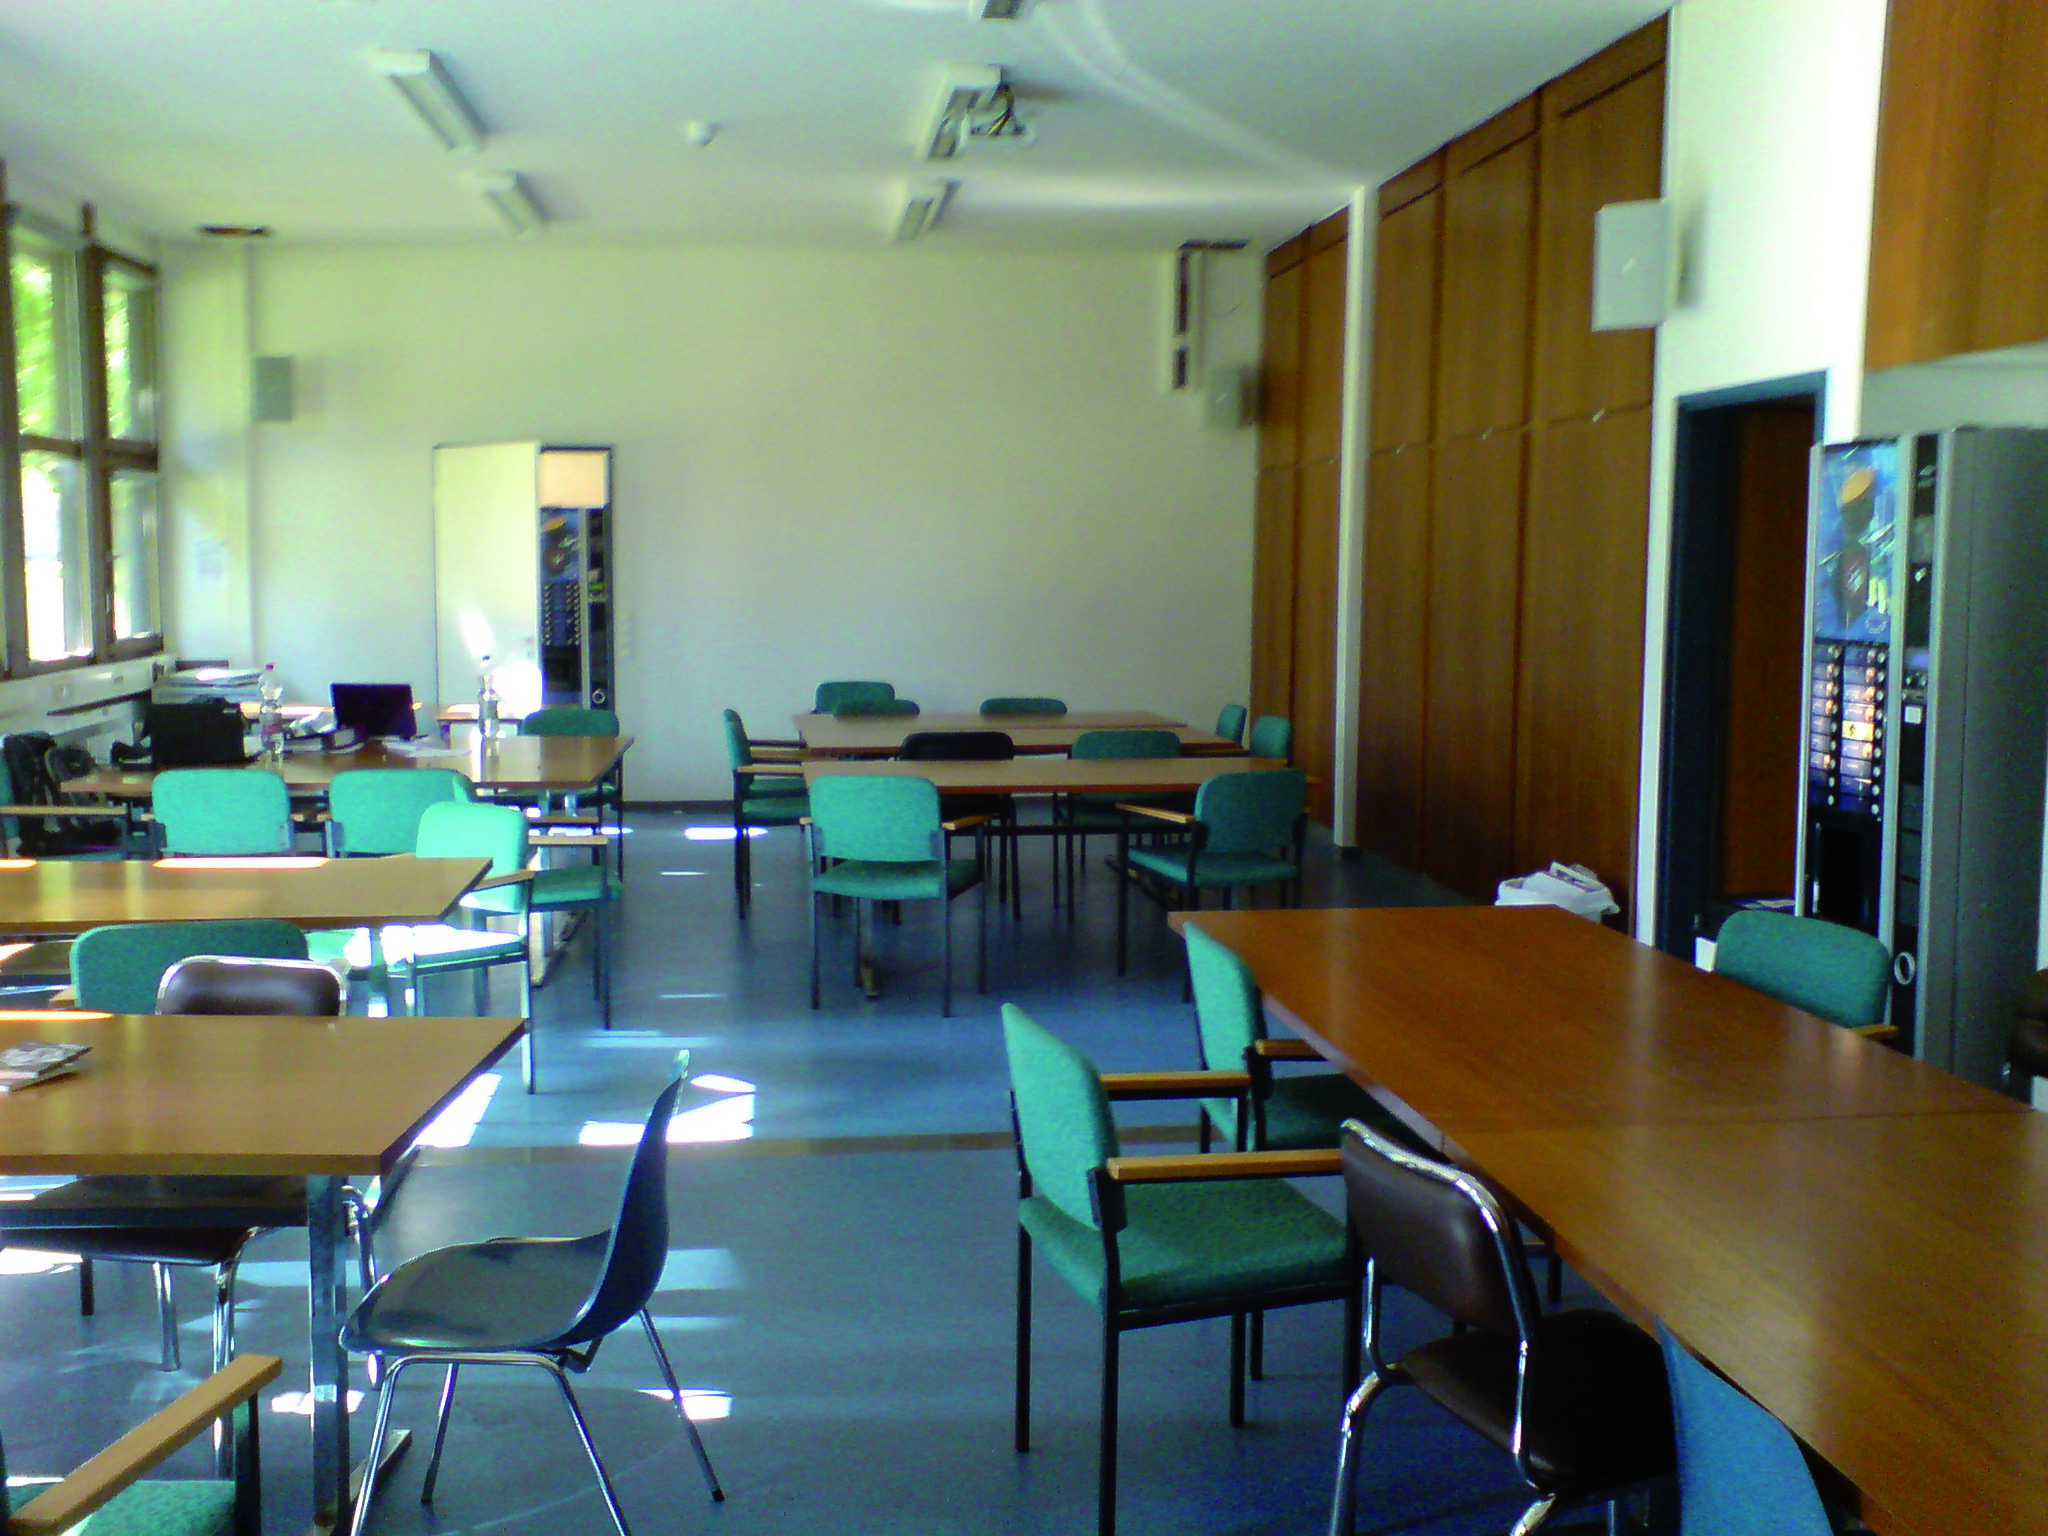
\includegraphics[width=\textwidth]{gumbel_raum_print}

\clearpage


\section{Hilfe und Beratung}

\subsection{Erste Hilfe: GAF}

Wir kennen nicht immer die Lösung, wissen dafür aber meistens, wer sie
kennt. Wir haben gute Kontakte zu vielen Institutionen und Personen an
dieser Uni. Wenn du uns einfach mal besuchen willst, bist du herzlich
willkommen. (Kontakt siehe \ref{gafKontakt}, S. \pageref{gafKontakt})

\subsection{Probleme mit Lehrveranstaltungen oder Lehrpersonal}

Die offizielle Ansprechstelle hierbei ist der Studiendekan deiner
Fakultät.  Er ist für die Qualität der Lehre verantwortlich. In jedem
Fall ist der sinnvollste Weg zu einer Lösung erst einmal das direkte
Gespräch mit dem Dozenten. Erst wenn ihr das Gefühl habt, ein Problem
lässt sich nicht anders lösen, bittet euren Studiendekan um
Hilfe. Oder fragt uns von der GAF.

\paragraph{Für die Fakultät 16 (Mathe, Info, Statistik)}\hfill\\
Prof. Werner Bley\\
Prof. Hans Jürgen Ohlbach\\
Prof. Thomas Augustin

\paragraph{Für die Fakultät 17 (Physik und Meteorologie)}\hfill\\
Prof. Erwin Frey

\subsection{Webforen}

In den Foren \url{die-informatiker.net}, \url{die-physiker.org}
und \url{die-mathematiker.net} kann man sich mit seinen Kommilitonen
(und teils auch Lehrpersonal) austauschen.


\subsection{Ansprechpartner}

Alle nachfolgenden Personen sind sehr umgängliche Menschen, mit denen
man bestens reden kann. Wie die meisten Professoren beißen sie nicht,
wenn man was zu beanstanden hat.

\paragraph{Mathematik (B.Sc., LA Gymnasium)}\hfill\\
Dr. Heribert Zenk (Heribert.Zenk@mathematik.uni-muenchen.de)\\
Theresienstr. 39, B333, Telefon: 089 / 2180\textendash 4460\\
Sprechstunde: Mo, 15:00\emd{}16:00~Uhr\\

Dr. Hartmut Weiß (hartmut.weiss@mathematik.uni-muenchen.de)\\
Theresienstr. 39, B317, Telefon: 089 / 2180\emd{}4680\\
Sprechstunde: Do, 15:00\emd{}16:00~Uhr

\paragraph{Wirtschaftsmathematik (B.Sc.)}\hfill\\
Prof. Dr. Gregor Svindland (studienberatung.wirtschaftsmathematik@math.lmu.de)\\
Theresienstr. 39, B231, Telefon: 809 / 2180\emd{}4628\\
Sprechstunde: nach Vereinbarung

\paragraph{Mathematik (LA Grund-, Haupt-, und Realschule)}\hfill\\
Dr. Erwin Schörner (schoerner@lmu.de)\\
Theresienstr. 39, B237, Telefon: 089 / 2180\emd{}4498\\
Sprechstunde: nach Vereinbarung

\paragraph{Mathematik (Fachdidaktik und Didaktik)}\hfill\\
Prof. Dr. Hedwig Gasteiger (gasteiger@math.lmu.de)\\
Theresienstr. 39, B215, Telefon: 089 / 2180\emd{}4631\\
Sprechstunde: nach Vereinbarung

\paragraph{Informatik (B.Sc.)}\hfill\\
Dr. Reinhold Letz (reinhold.letz@lmu.de)\\
Oettingenstr. 67, E001, Telefon: 089 / 2180\emd{}9693\\
Sprechstunde: Mo \& Do 13:00\emd{}14:00~Uhr und nach Vereinbarung

\paragraph{Informatik (LA)}\hfill\\
Prof. Martin Hofmann, PhD (lehramt@ifi.lmu.de)\\
Oettingenstr. 67, L107, Telefon: 089 / 2180\emd{}9341

\paragraph{Medieninformatik (B.Sc.)}\hfill\\
Max Maurer / Simon Stusak (studentenbetreuer@medien.ifi.lmu.de)\\
Amalienstr. 17, 505, Telefon: 089 / 2180\emd{}4654

\paragraph{Physik (B.Sc.)}\hfill\\
Dr. Jana Traupel (jana.traupel@physik.uni-muenchen.de)\\
Schellingstr. 4, H417, Telefon: 089 / 2180\emd{}5033

\paragraph{Physik plus Meteorologie (B.Sc.)}\hfill\\
Dipl. Met. Heinz Lösslein (loesslein@lmu.de)\\
Theresienstr. 37, A208, Telefon: 089 / 2180\emd{}4217

\paragraph{Physik (LA)}\hfill\\
Prof. Dr. Raimund Girwidz (girwidz@physik.uni-muenchen.de)\\
Theresienstr. 37, A012, Telefon: 089 / 2180\emd{}2020



\subsection{Prüfungsamt}
Die Prüfungsämter sind für alle Prüfungsangelegenheiten zuständig,
d.h. deine Noten, deine Praktika, deine Notenübersichten und
Abschlusszeugnisse etc. Sie sind bei der Fakultät zu finden, zu der
dein Studienfach gehört. Eine Zuordnung der Prüfungsämter zu den
einzelnen Studiengängen/-fächern findest du auf der Übersichtsseite
Studiengänge A--Z am unteren Ende der jeweiligen
Studiengangsinformationen.

\url{www.lmu.de/pruefungsaemter}

\clearpage

\subsection{Studentenkanzlei}

Die Studentenkanzlei muss wegen gewissen formalen Belangen
gelegentlich besucht werden. Der Besuch dieses kafkaesken Molochs ist
oft mit großen Wartezeiten und Unbill verbunden.  Es hilft, hartnäckig
zu bleiben und notfalls mehrfach zu kommen, bis man den richtigen
Sachbearbeiter trifft. Nicht umgehen lässt sich ein Besuch bei:

\begin{itemize}
\item Beantragen von Beurlaubungen (Krankheit, Ausland, Kinder\ldots)
\item Fragen zur Studienplatzvergabe/Immatrikulation (Anerkennung von Hochschulzugangsberechtigungen, nachträgliches Einschreiben, Verlust der Immatrikulationsbescheinigung)
\item Studienfachwechsel, zusätzliche Einschreibung für ein Doppelstudium
\item Bescheinigungen für die Krankenkasse, Rente, Quittungen für Studienbeiträge
\end{itemize}

HGB, E011 / E114\\
Mo, Di, Mi, Fr: 8:30 -- 11:30~Uhr, Do: 13:30 -- 15:00~Uhr\\
\url{www.lmu.de/studentenkanzlei}


\subsection{Gleichstellungsbeauftragte}

\url{www.gleichstellungsbeauftragte.lmu.de}

\subsection{Frauenbeauftragte der Fakultäten}

Fakultät 16 (Mathe, Info, Statistik): \newline
\url{www.mathematik-informatik-statistik.uni-muenchen.de/fakultaet/beauftragte/index.html}\\

Fakultät 17 (Physik, Meteorologie)\newline
\url{www.physik.uni-muenchen.de/fakultaet/einrichtungen/frauenbauftragte/index.html}

\subsection{Studieren mit Kind}

\ldots ist nicht unmöglich. Die Uni bietet z. B. diverse Betreuungsmöglichkeiten.

\begin{itemize}
	\item \url{studentenwerk-muenchen.de/studieren-mit-kind}
	\item \url{www.lmu.de/studium/beratung/beratung_service/beratung_lmu/schwangere_kind}
\end{itemize}

\subsection{Studieren mit Behinderung}

Solltest du aufgrund einer Behinderung, wie einer fachärztlich festgestellten Legasthenie, mehr Zeit, spezielle Hilfsmittel oder einen eigenen Raum für Klausuren benötigen, so kannst du beim Prüfungsamt einen Nachteilsausgleich beantragen.

\begin{itemize}
	\item \url{studentenwerk-muenchen.de/studieren-mit-behinderung}
	\item \url{www.lmu.de/barrierefrei}
\end{itemize}



\subsection{Kirchliche Beratung}
Die christlichen Hochschulgemeinden bieten neben ihrem konfessionellen Angebot auch überkonfessionelle psychologische Beratung und Aktivitäten (Ausflüge, Spieleabende).

\paragraph{Katholische Hochschulgemeinde (KHG)}\hfill\\
Leopoldstr. 11, Raum 205\\
\url{www.khg.lmu.de}

\paragraph{Evangelische Hochschulgemeinde (ESG)}\hfill\\
Friedrichstr. 25\\
\url{www.esg.lmu.de}



\subsection{Psychosoziale Beratung}

Wenn du das Gefühl hast, die Kontrolle zu verlieren, oder nicht nur fachlich mit
dem Studium und den Menschen um dich herum zurecht kommst:\\
www.studentenwerk-muenchen.de/beratungsnetzwerk/psychosoziale-und\newline -psychotherapeutische-beratung/


\subsection{Sonstige Beratung des Studentenwerks}
Helene-Mayer-Ring 9 (U3 Olympiazentrum)\\
\url{studentenwerk-muenchen.de/beratungsnetzwerk}

\begin{itemize}
	\item Allgemeine und Soziale Beratung
	\item Psychotherapeutische und Psychosoziale Beratungsstelle
	\item Studienkreditberatung
	\item Rechtsberatung
	\item Wohnungsberatung/ Privatzimmervermittlung
	\item Beratungsstelle „Sexuelle Belästigung, Diskriminierung und Gewalt“
	\item Beratung für ausländische Studierende
\end{itemize}



\clearpage

\section{Ausland und Praktika}

Auslandssemester oder -praktika machen sich immer gut im Lebenslauf,
und sind nebenbei bleibende Erinnerungen, von denen viele von uns mehr
profitiert haben als von der ein oder anderen Vorlesung.  Und falls du
dich für ein Thema besonders interessierst, bieten auch viele
Hochschulen im Ausland die Möglichkeit, eine Abschlussarbeit bei ihnen
zu verfassen bzw. verfassen zu lassen (\url{www.jura.uni-bayreuth.de}).

Hierbei wirst du Uni-intern vom \emph{Referat Internationale Angelegenheiten} und dem Career Center \emph{Student und Arbeitsmarkt} unterstützt, aber auch von Hochschulgruppen wie AISEC oder IAESTE (vom DAAD gefördert).

\subsection{Auslandsstudium}

Die LMU verfügt über eine Reihe von Partnerhochschule in aller
Welt. Der Austausch ist hier einfacher (Formalien, Anerkennung von
ECTS) und du wirst von den Studiengebühren befreit. Für die
Partnerhochschulen kann man sich nur ein Mal im Jahr bewerben, also am
besten frühzeitig über Fristen informieren und bewerben.
Ein Jahr vor der Abreise ist manchmal schon zu spät, um sich bei
allen Organisationen (insb. DAAD) zu bewerben.
Es ist aber auch möglich, sich selbst einen Austausch an einer anderen
Hochschule zu organisieren.

Falls du im Ausland erworbene ECTS an der LMU anerkennen lassen
möchtest, solltest du dies im Vorfeld mit dem Studiengangskoordinator
abklären.

Austauschabkommen und -verträge, sowie Erfahrungsberichte findest du unter:\\
\url{https://www.moveon.verwaltung.uni-muenchen.de/move/moveonline/exchanges/search.php?_language=de}

\subsection{Praktikum im In- und Ausland}

Neben Jobbörsen gibt es auch Datenbanken wie die des DAAD
(\url{eu-community.daad.de/index.php?id=38}) mit
Praktikums-Erfahrungsberichten. So kann man sich im Vorfeld schon
einen groben Überblick über das jeweilige Praktikum machen.

\subsection{Finanzierung}

Dies ist nur eine Auswahl der Möglichkeiten. Für bestimmte Länder und
Vorhaben gibt es auch noch spezielle finanzielle Unterstützungen. Die
Vorlaufzeit beträgt 3--18 Monate.

\begin{itemize}
\item Auslands-BAFöG: staatliche finanzielle Förderung (nicht zurückzuzahlen) für ein Studium oder Praktikum im Ausland. Hierbei sind auch viele förderungsberechtigt, die kein reguläres BAFöG erhalten, also auf jeden Fall bewerben!
\item ERASMUS: ein Stipendiumprogramm für ein 3- bis 12-monatiges Studium oder Praktikum im europäischen Ausland.
\item DAAD und PROSA LMU: Stipendien für Studium, Praktikum, Sprachkurse und Kurzprogramme im Ausland.
\end{itemize}

Referat Internationale Angelegenheiten\\
HGB, G013, Zugang über G011\\
Mo--Fr: 9:00--11.30~Uhr, Mi: 13:00--15:00~Uhr\\
\url{www.lmu.de/international/auslandsstudium}\\


Student und Arbeitsmarkt\\
HGB, G206\\
Mo, Di, Do und Fr: 10:00--12:00~Uhr\\
\url{www.s-a.lmu.de}


\clearpage

\section{Geld}

\subsection{Studienbeitrag}
Der Studienbeitrag setzt sich zusammen aus einem Beitrag an das Studentenwerk (42~€) und Studiengebühren (500~€).

\textbf{Frist für die Zahlung: 16. November 2012}

Von den Studiengebühren kann man sich befreien lassen mit einem der
folgenden Gründe:
\begin{itemize}
        \item Man hat mindestens zwei Geschwister, für die deine Familie
          Kindergeld bezieht
	\item Man hat einen Geschwisterteil, der Studiengebühren/-beiträge an einer Hochschule in der EU zahlt
	\item Man erzieht ein Kind
	\item Man ist chronisch krank
	\item Die Eltern haben extrem wenig Geld (unzumutbarer Härtefall)
	\item etc.
\end{itemize}

Die genauen Beschreibungen findet ihr unter: \url{www.lmu.de/studium/administratives/gebuehr/studiengebuehren/befreiungen/befreiungsgruende}

\textbf{Frist für die Befreiung: 31. Oktober 2012}

Wenn du zu den besten 10\% deines Jahrganges zählst, können dir die
Studiengebühren rückwirkend erlassen werden.

Sachgebiet 5 -- Studienbeiträge, HGB, E114\\
Mo, Di, Mi, Fr: 08:30 -- 11:30~Uhr, Do: 13:30 -- 15:00~Uhr\\
\url{www.lmu.de/studium/administratives/gebuehr/studiengebuehren}


\subsection{Jobben}
In München findest du eine Vielzahl an Nebenjobs: vom Café, Nachhilfe ($\geq$ 15~€/h) bis an der Uni selbst (ca. 9 -- 11~€/h). Deutlich höhere Stundenlöhne erhälst du, wenn du in einem der vielen IT-Unternehmen als Werkstudent arbeitest ($\geq$ 12~€/h).

Angebote findest du in Aushängen (Uni, Geschäfte) und Stadtmagazinen, aber auch unter den folgenden Adressen:
\begin{itemize}

\item in den Foren die-informatiker.net, die-physiker.org und die-mathematiker.net

\item \url{www.jobcafe.de}

\item \url{www.s-a.uni-muenchen.de/studierende/jobboerse/index.html}

\item \url{www.uni-muenchen.de/aktuelles/stellenangebote/stud_hilfskraft/index.html}
\end{itemize}

Beim Jobben solltest du den finanziellen Freibetrag der Krankenversicherung und ggf. beim BAFöG beachten, aber auch dass du unter den maximalen Wochenstunden bleibst (Krankenversicherung). Im Semester gelten dabei andere Grenzen als in den Semesterferien.

Dein Einkommen ist bis zu einer Grenze von ungefähr 8.000~€ (Freibetrag ohne Werbekosten etc.) steuerfrei.


\subsection{BAföG}
Im Studium kann man vom Staat finanzielle Unterstützung nach dem BundesAusbildungsförderungsGesetz erhalten. Grundsätzlich bekommen all diejenigen BAföG, die ihre Ausbildung nicht anderweitig finanzieren können (abhängig von deinem Einkommen und dem deiner Eltern / Fürsorgepflichtigen). Der Förderbetrag muss nach dem Studium zur Hälfte zurückgezahlt werden (zinsloses Darlehen), der Rest wird erlassen.

Einen ersten Eindruck von deiner Chancen auf BAföG bzw. die erwartbare
Höhe bekommst du mit dem BAföG-Rechner:
\url{www.bafoeg-rechner.de/Rechner}

Bei einem Nein im Rechner kann es trotzdem sein, dass du BAföG
bekommst. Überlege, ob sich der Aufwand des Einreichens und
Nachreichens der Anträge für dich lohnt.

Die Bafög-Unterlagen erhältst du unter: \url{das-neue-bafoeg.de}\\
oder kannst sie online ausfüllen unter: \url{bafoeg-bayern.de}

Für allgemeine Fragen kannst du dich an die allgemeine BAföG-Beratung des Studentenwerks wenden:

Helene-Mayer-Ring 9, Raum h4\\
Tel.: 089 357135-30\\
beratung-m@bafoegbayern.de\\
Mo, Di, Mi: 9:00--13:00~Uhr, 14:00--16:00~Uhr, Do: 9:00--13:00~Uhr, 14:00--17:00~Uhr, Fr: 9:00--13:00~Uhr

Konkrete Fragen besprichst du am Besten mit deinem Sachbearbeiter.

\subsection{Stipendien}
Stipendien haben meistens einen finanziellen und einen ideellen Anteil
(Seminare etc.). Für ein Stipendium ist neben passablen Noten vor
allem soziales Engagement wichtig.

\begin{itemize}
	\item Deutschland-Stipendium: \url{www.lmu.de/deutschlandstipendium}
	\item Sonstige Stipendien: \url{www.lmu.de/studium/studienfinanzierung/stift}
\end{itemize}

Es gibt diverse weitere Stipendien, die nicht nur auf Noten achten.
Suchen lohnt sich!

\clearpage

\section{Krankenversicherung für Studenten}

Für Studenten an staatlichen und staatlich anerkannten Hochschulen
besteht generell eine Kranken- und Pflegeversicherungspflicht. Diese
Pflicht beginnt mit der Immatrikulation an der Hochschule und endet in
der Regel nach Ablauf des 14. absolvierten Fachsemesters oder mit der
Vollendung des 30. Lebensjahres. Dabei sind verschiedene Formen der
Versicherung möglich.

\paragraph{Ich bin Student und meine Eltern sind gesetzlich krankenversichert}

Alle Studienanfänger, die weniger als 350\~€ im Monat verdienen, sind
bis zum Ende ihres 25. Lebensjahres über die Eltern in der
gesetzlichen Familienversicherung mitversichert. Für diejenigen, die
zwischen Abitur und Studienbeginn Zivil- oder Wehrdienst abgeleistet
haben, verlängert sich die Zeit in der Familienversicherung um die
Dauer des Dienstes. Während dieser Zeit muss man sich generell um
nichts kümmern – von der Bescheinigung über die Versicherung für die
Immatrikulation einmal abgesehen. Es besteht die Möglichkeit, sich
während der ersten drei Monate des Studiums nach Studienbeginn von der
gesetzlichen Krankenversicherung befreien zu lassen und sich privat zu
versichern.

\paragraph{Ich bin Student und meine Eltern sind privat krankenversichert}

Bei einer privaten Krankenversicherung gibt es die Möglichkeit, bis zu
seinem 25. Lebensjahr im Rahmen einer Familienversicherung
mitversichert zu sein. In der privaten Krankenversicherung muss
allerdings pro Familienmitglied ein bestimmter Betrag gezahlt
werden. Die kostenlose Familienversicherung gibt es nur in der
Gesetzlichen. Wenn man sich privat familienversichern will, muss man
sich innerhalb der ersten drei Monate des Studiums von der
studentischen Pflichtversicherung befreien lassen, was aber generell
kein all zu großer Aufwand ist. Man kann sich auch dafür entscheiden,
sich schon zu Studienbeginn gesetzlich über die studentische
Krankenversicherung zu versichern und damit aus der privaten
Familienversicherung auszutreten.

\paragraph{Ich bin Student und verdiene mehr als 350~€ im Monat}

Wer als Student mehr als 350~€ im Monat verdient, fällt aus der
Familienversicherung heraus. Eine Ausnahme stellen nur so genannte
Minijobs dar, bei denen die Verdienstgrenze auf 400~€ angehoben
wird. Wer diese Grenze nur sehr knapp überschreitet, sollte vor
Studienbeginn noch einmal genau nachrechnen: Bei der Rechnung zur
Krankenversicherung kann die so genannte Werbungskostenpauschale
geltend gemacht werden, mit der man noch einmal etwas mehr als 70~€
vom Monatsgehalt abziehen kann. Wer immer noch oberhalb der
Einkommensgrenze liegt, kann zwischen einer gesetzlichen und privaten
Krankenversicherung wählen.

\paragraph{Ich bin Student und über 25}

Sofern sich die Altersgrenze nicht durch das Ableisten eines Wehr-
oder Zivildienstes nach hinten verschoben hat, endet mit dem
26. Geburtstag die Mitgliedschaft in der Familienversicherung. Dann
kann man sich gleich zu Studienbeginn über die studentische
Krankenversicherung versichern. Nach Vollendung des 30. Lebensjahres
oder nach dem 14. Fachsemester hat man außerdem die Möglichkeit sich
von der Versicherungspflicht zu befreien.

\paragraph{Ich bin Student und über 30}

Mit dem 31. Geburtstag erlischt auch die Möglichkeit der
Mitgliedschaft in der studentischen gesetzlichen
Krankenversicherung. Nach Ablauf dieser Frist kann man sich als
Student trotz Pflichtversicherung als freiwilliges Mitglied in der
Krankenversicherung einstufen lassen und bezahlt dann einen etwas
günstigeren Monatssatz von etwa 120~€. Dies ist aber nur möglich, wenn
man vorher auch gesetzlich versichert war. Bei der privaten
studentischen Krankenversicherung liegt die Altersobergrenze bei 34
Jahren. Allerdings gibt es hier anschließend nicht die Möglichkeit den
Freiwilligenstatus einzunehmen.

\paragraph{Studenten-Krankenversicherung in der gesetzlichen Krankenkasse}

Die Beitragssätze sind bei allen Krankenkassen gleich (ca. 80~€ im
Monat). Unterschiede gibt es bei den einzelnen Kassen aber oft im
Leistungsumfang, so dass ein Vergleich lohnt. Da die Krankenkassen bei
Studierenden auf künftig gut verdienende Mitglieder hoffen, werden
diese an den Hochschulen manchmal regelrecht umworben. Dementsprechend
sind die angebotenen Leistungen der Krankenkassen meist nicht
schlecht.

\paragraph{Studenten-Krankenversicherung in der privaten Krankenkasse}

Natürlich sind auch die privaten Versicherer daran interessiert,
Mitglieder aus dem akademischen Bereich zu generieren. Und so sind die
Konditionen der privaten Studenten-KV meist recht gut. Zudem ist der
Leistungsumfang üblicherweise wesentlich höher. Vor allem für
männliche Studenten kann sich der Abschluss einer privaten
Studentenkrankenversicherung finanziell durchaus lohnen. Für weibliche
Versicherungspflichtige sind die Tarife der
Studenten-Krankenversicherung meist höher, können aber unter
bestimmten Umständen trotzdem attraktiv sein. Das kann etwa der Fall
sein, wenn das Einkommen hoch genug ist um in der gesetzlichen
Krankenkasse zusätzlich beitragspflichtig zu sein.

Die private Studenten-KV hat aber auch Nachteile. So ist es nach
Abschluss des Studiums meist schwierig und unter Umständen auch gar
nicht möglich, wieder in eine gesetzliche Krankenkasse zu
wechseln. Nötig ist dazu das dauerhafte Absinken des Einkommens unter
die Versicherungspflichtgrenze (knapp 50.000~€). Bei den Privaten sind
die Tarife meist in jungen Jahren günstig und steigen später deutlich
an. Wer später die günstigeren Tarife der Gesetzlichen nutzen möchte,
soll sich dem Solidarprinzip hier nicht im Vorfeld entziehen. Dies ist
zumindest der Standpunkt der Gesetzgeber.

\footnotesize (zusammengestellt aus {\url{studenten-krankenversicherung.net}})
\normalsize

\clearpage

\section{Ankommen in München}

\subsection{Ummeldung / Zweitwohnsitz}
\begin{itemize}
	\item Ort: \url{muenchen.de/dienstleistungsfinder/muenchen/1063475/}
	\item Zweitwohnungsteuer: 9 \% der jährlichen Nettokaltmiete
	\item Befreiung Zweitwohnsitzsteuer: Nachweis über positive Einkünfte unter 25.000~€ (z.B. BAföG-Bescheid) bis 31.1. \newline (\url{muenchen.de/Rathaus/ska/fachinfos/zweitwohnst/einkommensabhaengig.html})
\end{itemize}

\subsection{Mülltrennung}
\begin{itemize}
	\item Trennung nach: Restmüll, Papier, (Bio,) Plastik, Dosen, Altglas und den üblichen Sachen wie Sperrmüll, Elektroschrott u.ä.
	\item Für Plastik, Dosen und Altglas gibt es Container, die über die Stadt verteilt sind
	\item \url{awm-muenchen.de}
\end{itemize}

%\subsection{Wohnung}
%\begin{itemize}
%	\item Die beliebtesten Portale für WGs: \url{wg-gesucht.de} und \url{studenten-wg.de} (Wenn ihr euch bewerbt, schreibt mehr als euren Namen und Telefonnummer.  Stellt euch persönlich vor, bringt Bier mit ;-)).
%	\item Wohnheim: \url{studentenwerk-muenchen.de/wohnen}
%	\item andere Angebote: \url{studentenwerk-muenchen.de/wohnen/weitere-wohnangebote}
%	\item Notunterkünfte: \url{www.caritastoelz.de/Page010179.htm}, \url{www.wohnhilfe-muenchen.de/jugendhilfe/die-jugendpension-jup.html}
%\end{itemize}

\subsection{GEZ}
\begin{itemize}
	\item Nach der Ummeldung wirst du wahrscheinlich bald Post von der GEZ bekommen.
	\item Befreiung möglich, wenn du BAföG bekommst (Antrag stellen)
	\item Gebühren Radio, Computer: 5,76~€/Monat \\
Gebühren Radio, Computer, Fernseher: 17,98~€/Monat
        \item \url{gez.de}
        \item http://www.lawblog.de/index.php/archives/2011/04/15/generelles-hausverbot-fr\newline -gez-mitarbeiter-mglich/
\end{itemize}

\subsection{Rundfunkbeitrag}
\begin{itemize}
    \item ab 1.1.2013
    \item 17,98~€/Monat pro Haushalt unabhängig von den Geräten
    \item Befreiungsantrag ab November möglich
    \item \url{rundfunkbeitrag.de}
\end{itemize}

\subsection{Wohnen}
Teuer, schwer zu bekommen und hart umkämpft. Die Mietpreise liegen
auch für Studenten ca. 50--100~€ über dem üblichen mittleren Preis in
Restdeutschland. Das Studentenwerk bietet auf seiner Homepage eine
gute Übersicht über

\begin{itemize}
\item Studentenwerkswohnheime \newline \url{studentenwerk-muenchen.de/wohnen/wohnanlagen-des-studentenwerks-muenchen/}

  günstig aber schwer zu bekommen (erkundigt euch in den Verwaltungstellen direkt)
\item private Wohnheime, oft in eigener oder karitativer Trägerschaft
  (Bewerbungen sind nötig, z. T. gibt es Bedingungen, der Versuch lohnt sich)
\item
  Privatzimmer \newline \url{http://www.studentenwerk-muenchen.de/wohnen/vermittlung-von-privatzimmern/}
  
werden vom Studentenwerk und der Mitwohnzentrale vermittelt.
\item Wohnen gegen Hilfe für ältere Leute, die der helfenden Hand dafür
  Wohnraum stellen.
\item andere Angebote: \url{studentenwerk-muenchen.de/wohnen/weitere-wohnangebote}
\item {\bf Notunterkünfte}, falls alles schiefgeht:

 \url{www.caritastoelz.de/Page010179.htm},

  \url{www.wohnhilfe-muenchen.de/jugendhilfe/die-jugendpension-jup.html}
\end{itemize}

\paragraph{WGs gibt es reichlich, sucht hier:}
\url{wg-gesucht.de} und \url{studenten-wg.de}\newline
Eine freundliche E-Mail mit einer Vorstellung Eurer selbst und warum ihr
in diese WG passt ist wichtig.

\paragraph{Selbst mieten} ist teuer, aufwändig und oft sind Provisionen
fällig. Die Mieten sind in den letzten Jahren nochmal kräftig gewachsen.
Suchen
lohnt sich in den gängigen Online Portalen und auf der Immobilienseite der
Süddeutschen Zeitung, auch online. Meistens werden Bürgschaften oder andere
Sicherheiten verlangt.  Wer vorbereitet zur Besichtigung kommt, ist im Vorteil.

\clearpage

\section{Fortbewegung}

\subsection{Fahrrad}

Fahrradfahren lohnt sich nicht nur, weil es die schnellste und
flexibelste Möglichkeit ist, in München voranzukommen, es ist auch
gesund, schont das Klima und macht Spaß.  Es ist auch deutlich
günstiger als die häufig überfüllten öffentlichen Nahverkehrsmittel:
Drei Monate Fahrrad statt MVG und schon hast du mindestens 100~€
gespart.

Damit kann man schon den ein oder anderen Drahtesel refinanzieren oder
hat zumindest eine Anzahlung für ein gutes, gebrauchtes Fahrrad. Diese
findet man beispielsweise bei eBay, Polizei-, Bahnhofs- und
Wohnheimversteigerungen oder auf einem der zahlreichen Flohmärkte in
München. Kleiner Tipp: Beschränke dich bei der Suche nicht nur auf die
Stadt, sondern beziehe das Umland mit ein. Dort findet man oft
deutlich bessere Angebote.

\paragraph{Hier noch ein paar Tipps für den Münchner Straßenverkehr:}
\begin{itemize}
	\item Um Trambahnschienen sollte man nicht nur bei Regen und Glätte einen großen Bogen machen.
	\item Fußgänger sind in ihrem Verhalten unvorhersehbar. Die Autofahrer leider auch.
	\item Mit Licht und Helm fahren kann dein Leben retten.
	\item Um das Wiederfinden des Fahrrades zu erleichtern, sollte man es abschließen.
	\item München ist nicht nur Radlhauptstadt, sondern auch (gefühlte) Kontrollierhauptstadt:

	\begin{itemize}
        	\item Auf der richtigen Straßenseite fahren -- insbesondere auf der Leopold- / Ludwigstr. (15~€).
	        \item Nicht bei Rot über die Ampel fahren (min. 90~€ und ein paar Punkte in Flensburg).
	        \item In der Innenstadt Schrittgeschwindigkeit einhalten, wo es ausgeschildert ist (15~€).
	        \item Nicht ohne Licht durch Nacht und Dunkelheit (15~€).
	\end{itemize}
\end{itemize}

%\begin{textblock*}{\paperwidth}(50mm,128mm)
%   \noindent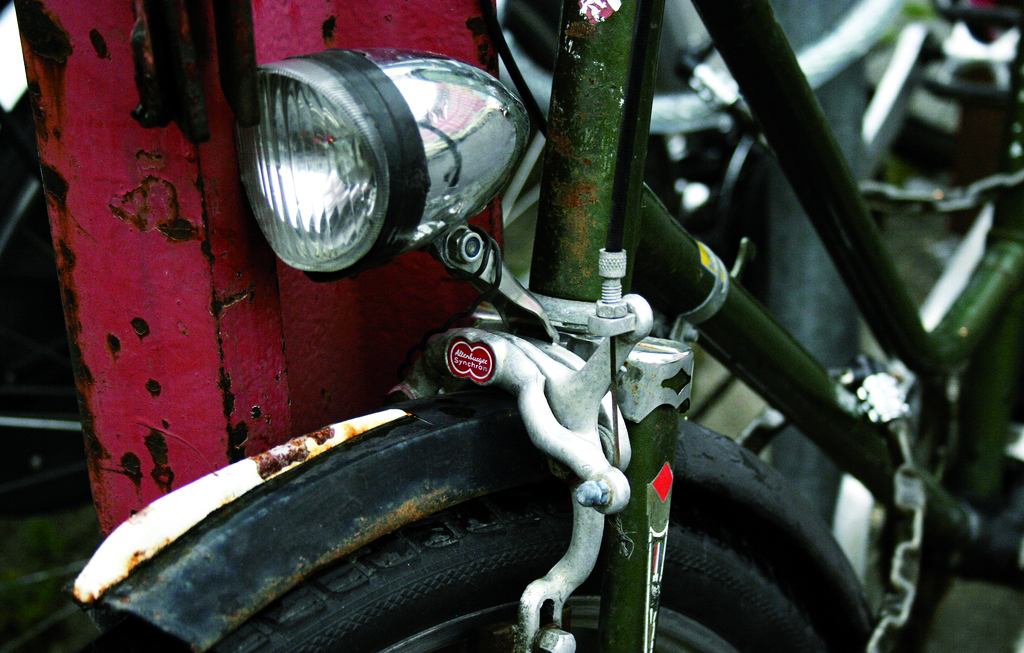
\includegraphics[width={\paperwidth-50mm}]{flickr/725703538_5b9a97ecf2_b}
%	\label{img_bike}
%\end{textblock*}

\clearpage

\subsection{MVV}

\paragraph{Mit den öffentlichen Verkehrsmitteln in die Uni}\hfill\\
Mit der U3 bzw. U6 Haltestelle Universität kommst du direkt zum Hauptgebäude. Zu den meisten anderen Gebäuden kommst du von dort aus relativ schnell. Für diese gibt es aber meistens auch näherliegende Haltestellen, welche man auch auf der Karte in diesem Heft finden kann.

\paragraph{Kosten}\hfill\\
Für die meisten Studenten ist momentan der von der MVV (Münchner Verkehrsverbund) angebotene Ausbildungstarif II am interessantesten. Der Preis richtet sich dabei nach der Zahl der benötigten Zeitkartenringe, die befahren werden. Bevor du dir aber ein Ticket kaufen kannst, musst du dir ein Kundenkarte besorgen. Diese bekommst du im MVG-Kundencenter am Hauptbahnhof, Ostbahnhof oder in der Poccistr.~1--3 (alle zwischen 8:00 und 18:00~Uhr) oder online \newline http://www.mvv-muenchen.de/de/tickets-preise/tickets/schule-ausbildung-und-studium/\newline kundenkarte/index.html\#c9815

Das Ticket gibt es mit der Gültigkeit einer Woche (9,50 -- 38,90~€) oder eines Monats (34,70 -- 142,00~€) an einem der MVG-Zeitkartenautomaten, in den MVG-Kundencentern oder den MVG-Verkaufsstellen. Monatsfahrkarten gelten bis 12Uhr des ersten Werktags des Folgemonats.\\
~
Wenn du in Zukunft günstiger unterwegs sein willst, kannst du bei der Initiative Ausbildungsticket, einem Bündnis aus Studenten, Schülern und Azubis mitmachen:\newline \url{ausbildungsticket.de}

Mehr Infos zum Ausbildungstarif: \url{mvg-mobil.de/tarife/ausbildungstarif.html}


\subsection{Auto}
Du kommst im Allgemeinen mit dem Auto nicht schneller durch die Stadt, als mit dem ÖPNV oder dem Fahrrad. Spätestens bei der Parkplatzsuche vor der Uni wirst du dann merken, dass es bessere Möglichkeiten gibt, an die Uni zu kommen.

\pagebreak

\section{Gebäudeübersichten}

\subsection{Theresienstr. -- Mathebau}

\begin{center}
\bf Erdgeschoss \hspace{0.5\textwidth} 1. Stock

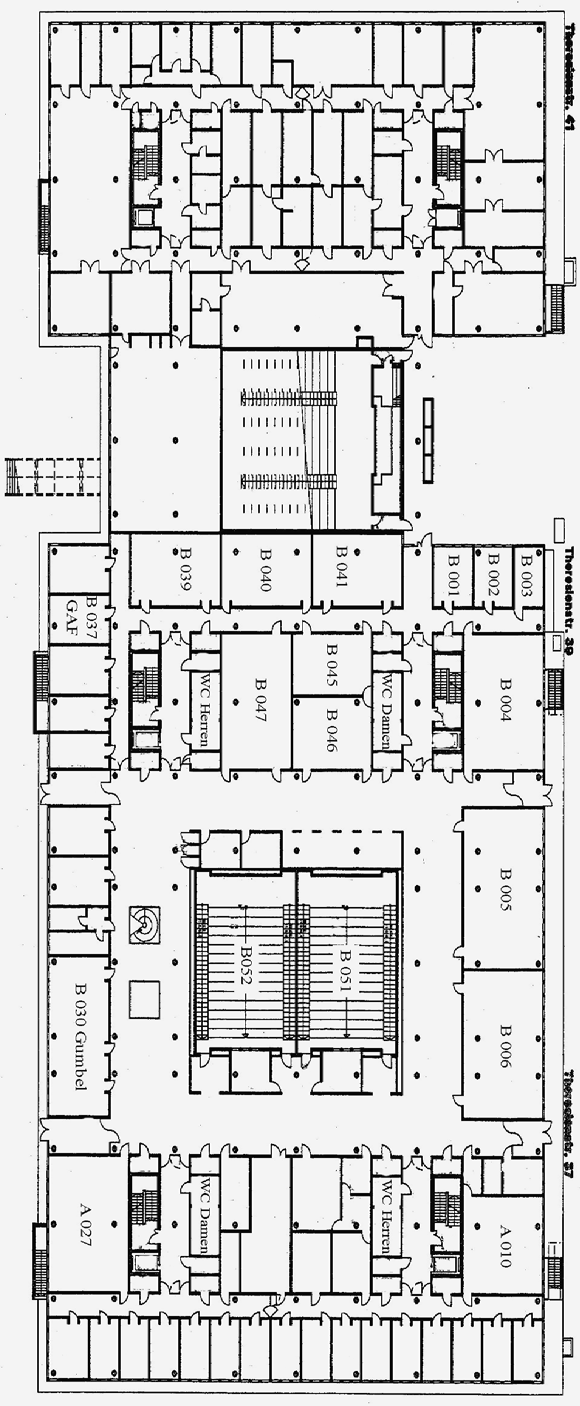
\includegraphics[width=0.49\textwidth]{theresien1.png}
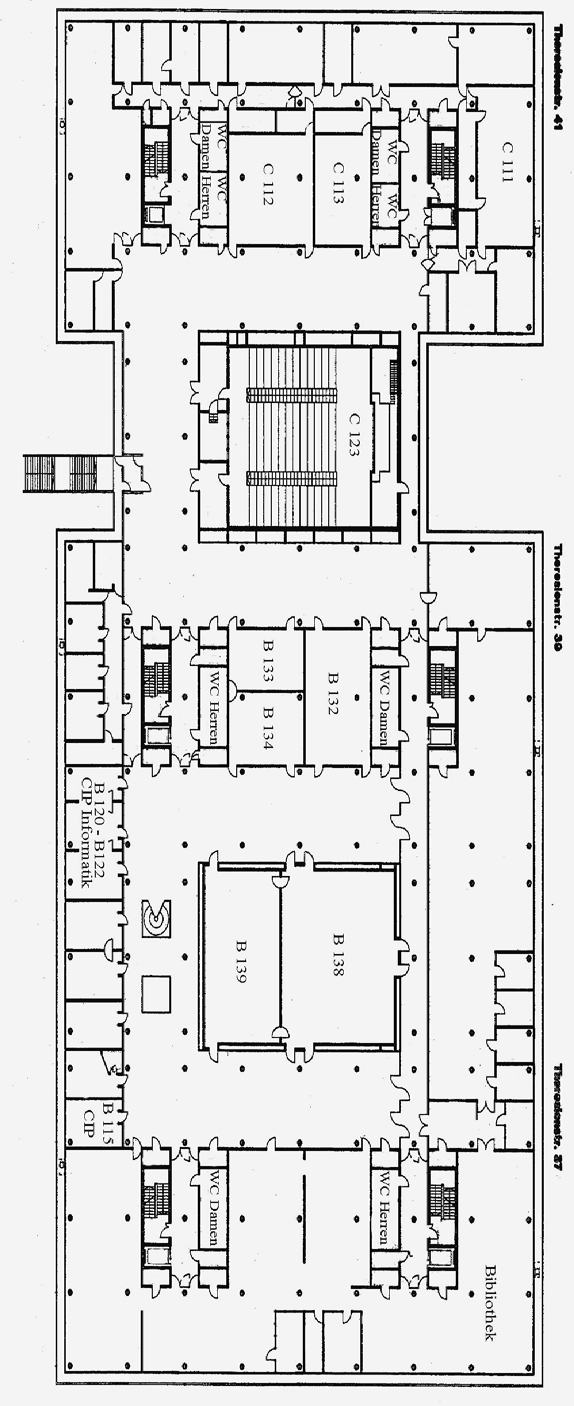
\includegraphics[width=0.49\textwidth]{theresien2.png}


\subsection{Oettingenstraße -- Erdgeschoss}

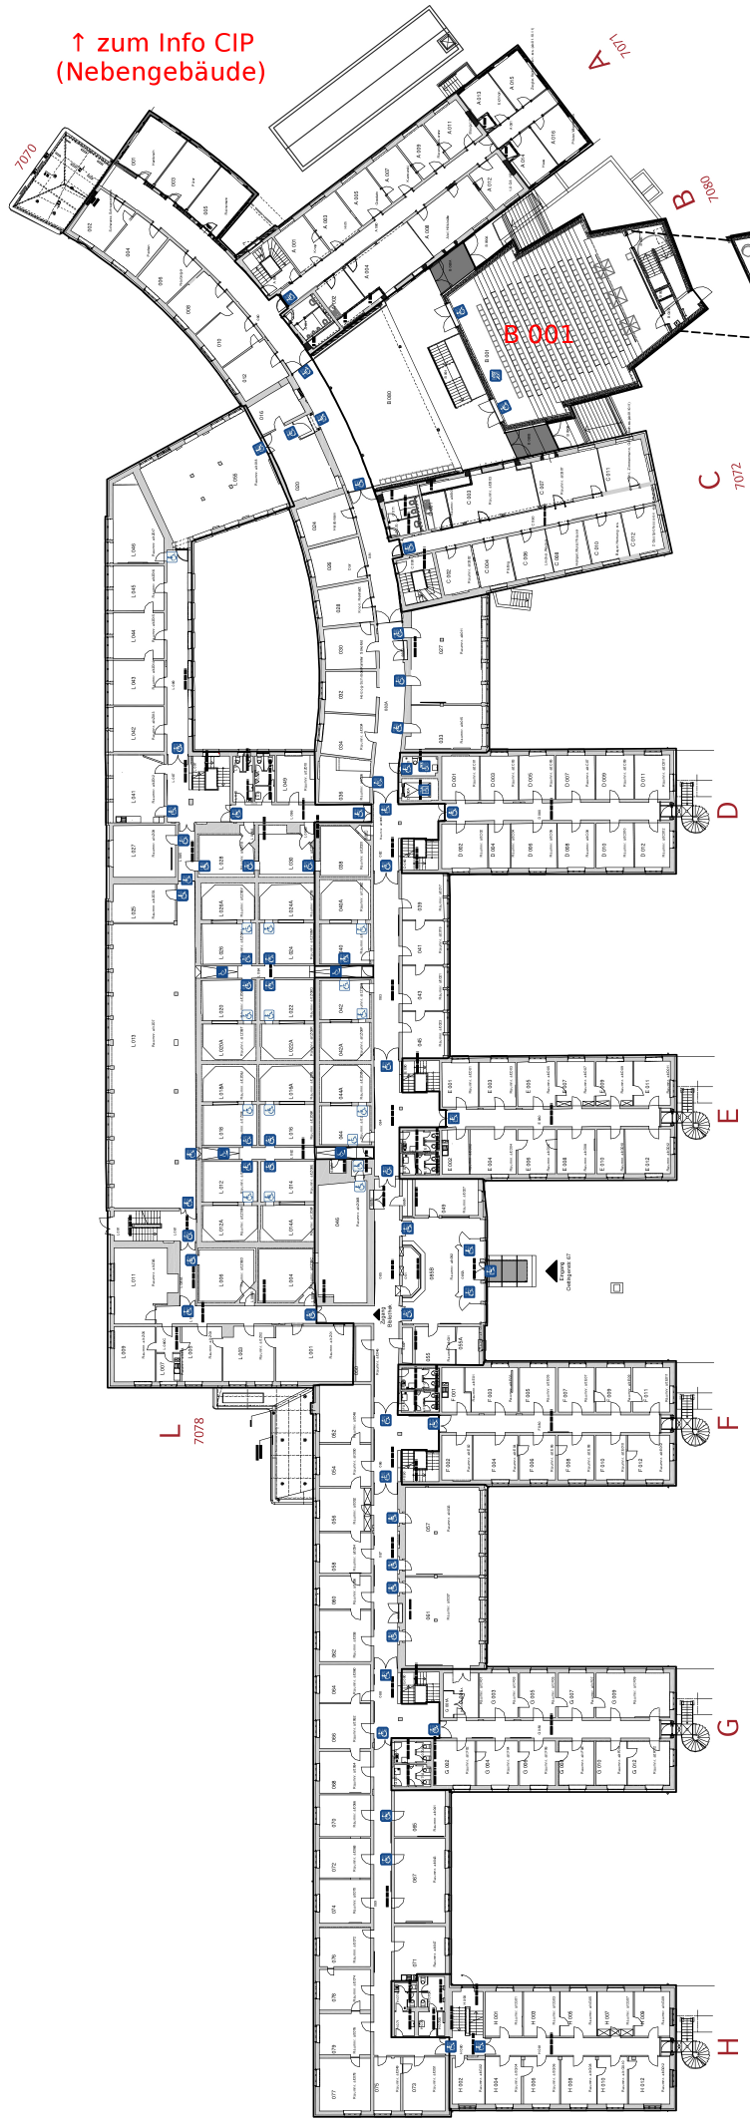
\includegraphics[height=0.9\textheight]{oettingen.png}

\subsection{Schellingstr. 4 -- Physik}


\includegraphics[width=0.5\textwidth]{schelling.png}

\subsection{Hauptgebäude}

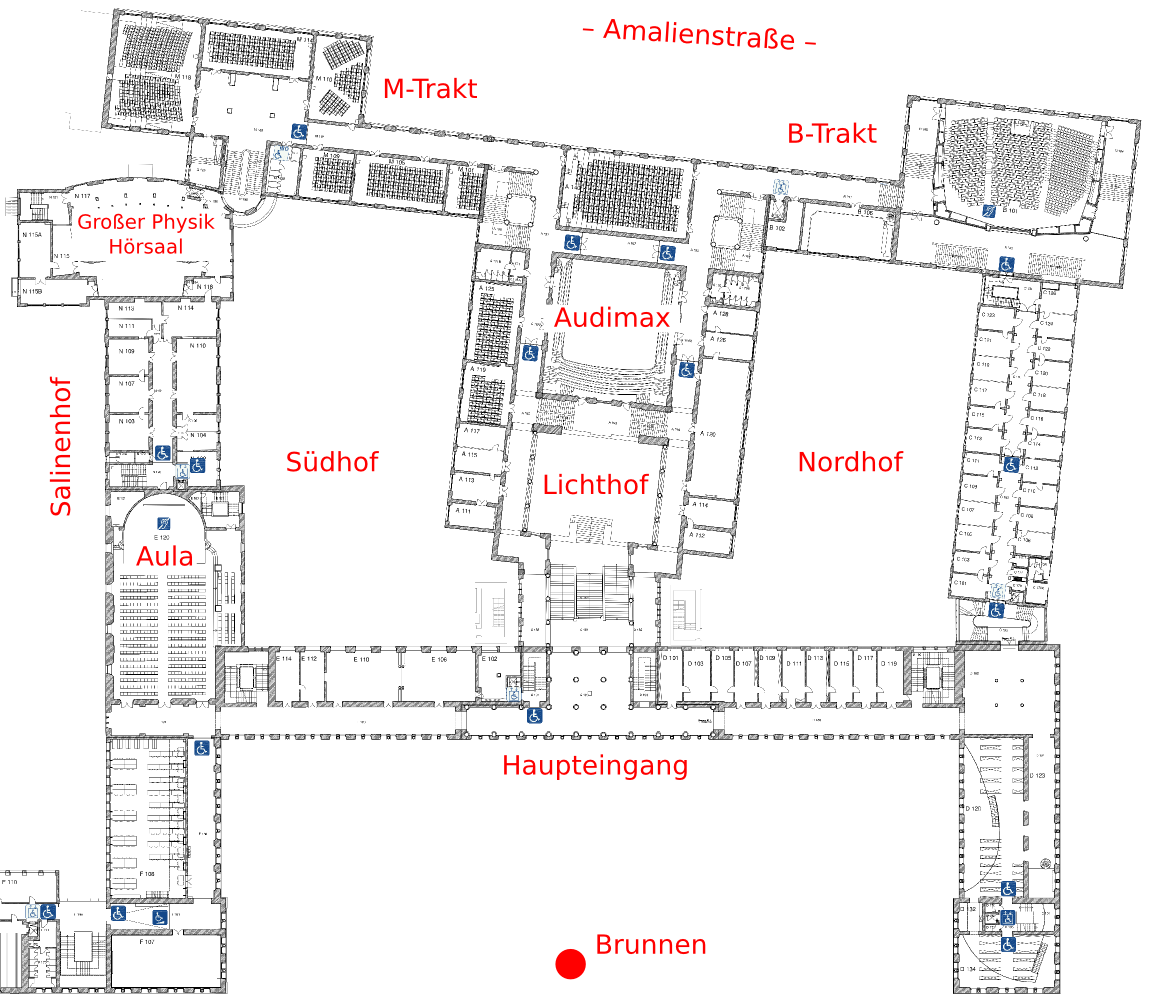
\includegraphics[height=0.6\textheight]{hauptgeb.png}

\end{center}

\begin{multicols}{2}
\setlength{\parindent}{0pt}

\pagebreak
\section{Rätselseite}

\textbf{Mini-Sudoku}: Trage in jede Zeile und Spalte
  die Ziffern 1, 2, 3,~4 so ein, dass A~waagrecht, A~senkrecht,
  B~senkrecht und F~senkrecht Primzahlen sind!\\[0.2cm]
\begin{tabular}{ |p{0.8cm}|p{0.8cm}|p{0.8cm}|p{0.8cm}| }
\hline
  a & b & c & d \\[0.8cm]
\hline
  e &   &   &   \\[0.8cm]
\hline
  f &   &   &   \\[0.8cm]
\hline
  g &   &   &   \\[0.8cm]
\hline
\end{tabular}

\medskip
\textbf{Löse folgende Gleichung:}

\[\frac{\textrm{EVE}}{\textrm{D\,I\,D}} = \textrm{0,TALKTALKTALK}\dots\]

Jeder Buchstabe steht für eine andere Ziffer.

\textbf{Visitenkarten:} Welchen Beruf haben diese Personen?\\

\centerline{Hanne Rubbich \textendash{} Ilztal\\[0.2cm]}
\centerline{Richie Hersvogt \textendash{} Zell\\[0.2cm]}
\centerline{Meike Schmettelin \textendash{} Berlin\\[0.2cm]}

\medskip
\textbf{Minesweeper:} Kennst du.  Jedes Level ist eindeutig lösbar.\\[0.2cm]
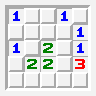
\includegraphics[width=0.45\linewidth]{minepuzzle_gen02tr.png}
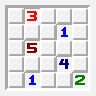
\includegraphics[width=0.45\linewidth]{minepuzzle_gen14tr.png}

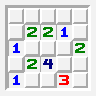
\includegraphics[width=0.45\linewidth]{minepuzzle_gen18tr.png}
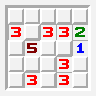
\includegraphics[width=0.45\linewidth]{minepuzzle_gen21tr.png}

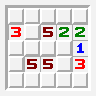
\includegraphics[width=0.45\linewidth]{minepuzzle_gen29tr.png}
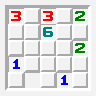
\includegraphics[width=0.45\linewidth]{minepuzzle_gen19tr.png}

\bigskip
\textbf{Kreuzzahlenrätsel:} Jede Summe, und jeder Summand innerhalb der Summe, darf nur einmal auftreten.

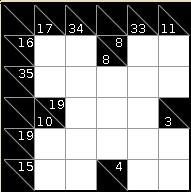
\includegraphics[width=0.9\linewidth]{2011-10-02-134837_191x192_scrot.png}

\end{multicols}

\clearpage

\section[Abkürzungen]{Häufig gebrauchte Abkürzungen}
\begin{tabular}{l p{10cm}}
BAföG        &Bundesausbildungsförderungsgesetz\\
c.t.        &Lat.: cum tempore (15 min später als angegeben)\\
EWO        &Erstsemesterwochenende\\
GAF        &Gruppe aktiver Fachschaftika\\
g.d.w.    & genau dann wenn\\
LMU        &Ludwig-Maximilians-Universität\\
LPO        &Lehramtsprüfungsordnung\\
LRZ        &Leibniz-Rechenzentrum\\
MVG    &Münchner Verkehrsgesellschaft\\
MVV    &Münchner Verkehrs- und Tarifverbund = \newline MVG + S-Bahn + $\Sigma$ Regionale Busunternehmen\\
N.N.        &Lat.: Nomen nominandus (noch zu nennen)\\
o.B.d.A.    &ohne Beschränkung der Allgemeinheit\\
RBG        &Rechnerbetriebsgruppe\\
RGB             &Rot-Grün-Blau\\
RTFM        &Read The Fucking Manual\\
s.t.        &Lat.: sine tempore (pünktlicher Beginn)\\
StuVe           &Studikavertretung\\
TUM/TU        &Technische Universität München\\
FH/HM        &[Fach-]Hochschule München\\
ZHS        &Zentraler Hochschulsport\\
\end{tabular}




\clearpage


\thispagestyle{empty}
\begin{textblock*}{\paperwidth}(0mm,0mm)
   \noindent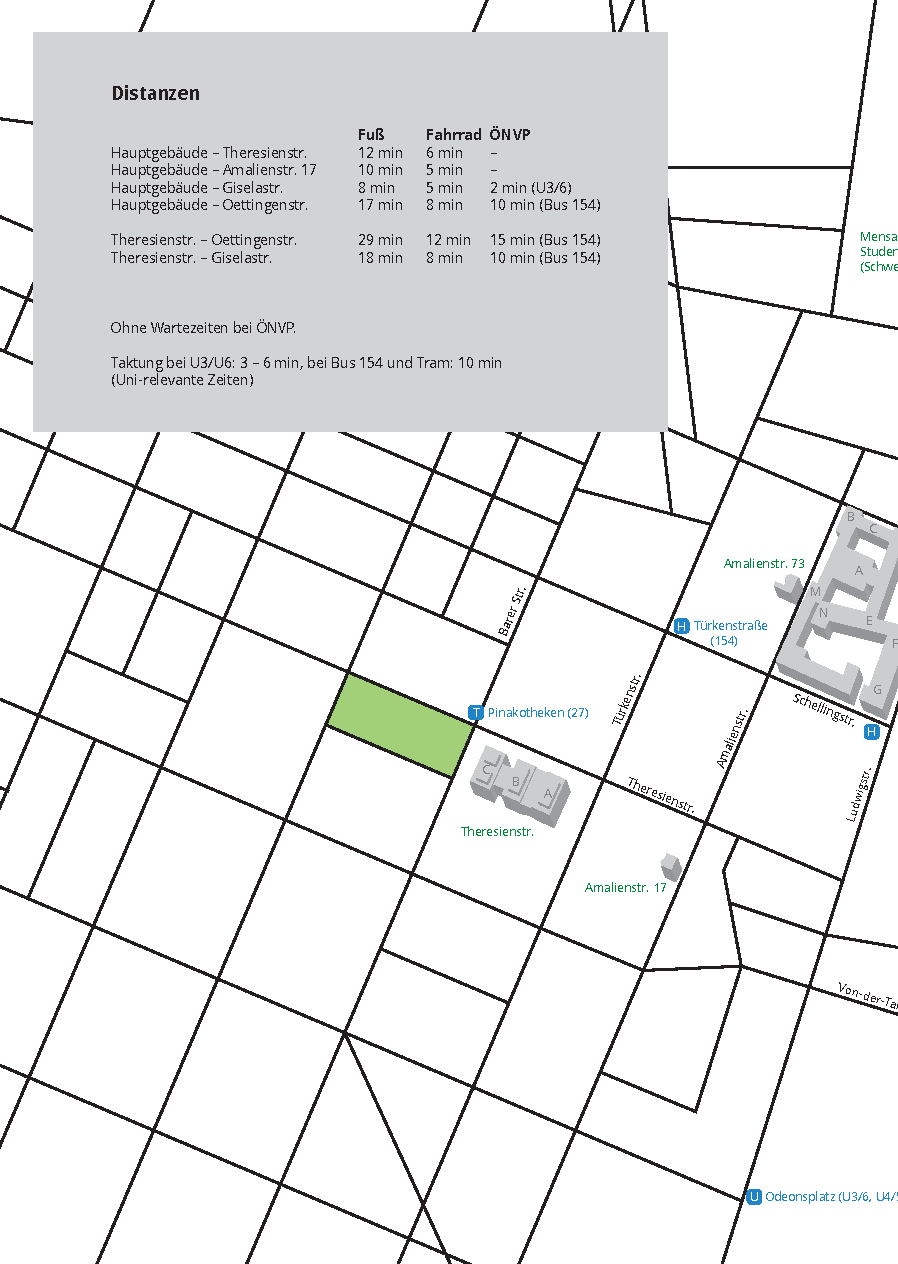
\includegraphics[width=\paperwidth,height=\paperheight]{lageplan_links}
\end{textblock*}
\mbox{}

\clearpage

\thispagestyle{empty}
\begin{textblock*}{\paperwidth}(0mm,0mm)
   \noindent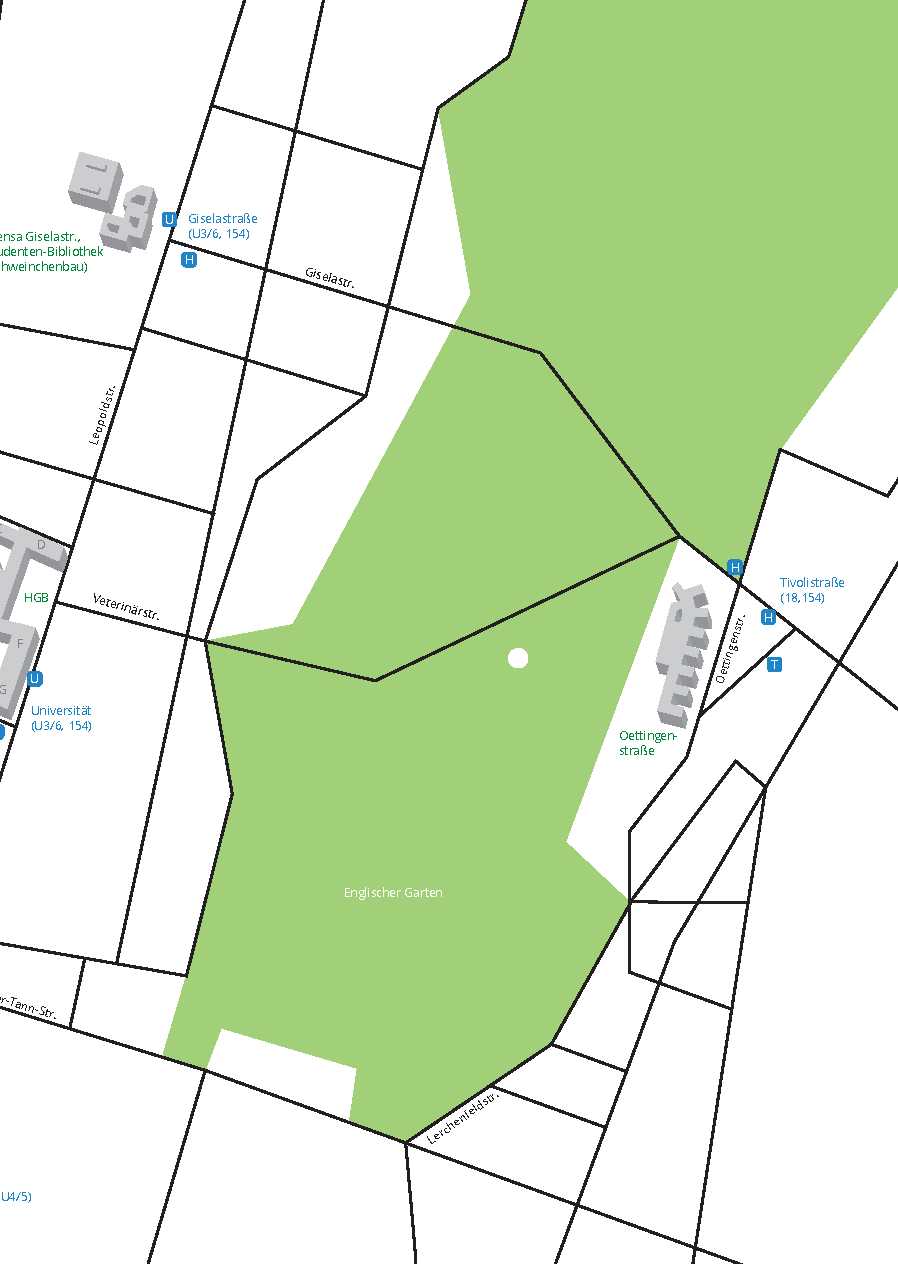
\includegraphics[width=\paperwidth,height=\paperheight]{lageplan_rechts}
\end{textblock*}
\mbox{}


\clearpage

\thispagestyle{empty}
\begin{textblock*}{\paperwidth}(0mm,0mm)
   \noindent
\includegraphics[width=\paperwidth,height=\paperheight]{back}
\end{textblock*}
\mbox{}




\end{document}
